\documentclass[11pt,a4paper]{report}

% Aberstwyth dissertation LaTeX Template
% Authors: Dr. Hannah Dee (hmd1@aber.ac.uk), Neil Taylor (nst@aber.ac.uk)
% This has been adapted from the Leeds Thesis template and the 
% Group Project template for Computer Science in Aberystywth University.
% 
% All comments and suggestions welcome.
%
% Template designed to be used with pdflatex: it may need alteration to
% run with a different LaTeX engine

% To build document on the unix command line, run four commands:
 
% pdflatex dissertation
% bibtex dissertation
% pdflatex dissertation
% pdflatex dissertation

% you will end up with dissertation.pdf 
\usepackage{mmp}

% the following packages are used for citations - You only need to include one. 
%
% Use the cite package if you are using the numeric style (e.g. IEEEannot). 
% Use the natbib package if you are using the author-date style (e.g. authordate2annot). 
% Only use one of these and comment out the other one. 
\usepackage{cite}
%\usepackage{natbib}

\usepackage{listings} %for code
\usepackage{caption}%for code captions
\usepackage{color} %for code
\usepackage{gensymb} %for degree symbol

% defines how code will be shown
\definecolor{dkgreen}{rgb}{0,0.6,0}
\definecolor{gray}{rgb}{0.5,0.5,0.5}
\definecolor{mauve}{rgb}{0.58,0,0.82}
% still code
\lstset{frame=tb,
  language=C, %Java
  aboveskip=3mm,
  belowskip=3mm,
  showstringspaces=false,
  columns=flexible,
  basicstyle={\small\ttfamily},
  numbers=none,
  numberstyle=\tiny\color{gray},
  keywordstyle=\color{blue},
  commentstyle=\color{dkgreen},
  stringstyle=\color{mauve},
  breaklines=true,
  breakatwhitespace=true
  tabsize=3
}
\graphicspath{{./figures/}}

% Use the following to selectively exclude chapters
%\includeonly{cover,abstract,acknowledge,declare,chapter1,chapter2}

\begin{document}


% all of the include directives below refer to tex files
% so 
\title{Odometry based Map Building}

% Your name
\author{Stefan Klaus}

% Your email 
\authoremail{stk4@aber.ac.uk}

\degreeschemecode{GH76} %e.g. G400 
\degreeschemetitle{AI \& Robotics,} % e.g. Computer Science
\degreetype{BSc}

\modulecode{CS39440} % i.e. CS39440, CC39440, CS39620
\moduletitle{Major Project} % i.e. Major Project or Minor Project

\date{21st April 2012} % i.e. the date of this version of the report

\status{Release} % Use draft until you create the release version. Then, change this to Release.
\version{1.0}

%The title and name of your supervisor.
\supervisor{Dr. Myra Wilson} 

%The email for your supervisor. 
\supervisoremail{mxw@aber.ac.uk}

\maketitle



 includes cover.tex - to change the content,
% edit the tex file

\pagenumbering{roman}

% This is the front page

\title{Odometry based Map Building}

% Your name
\author{Stefan Klaus}

% Your email 
\authoremail{stk4@aber.ac.uk}

\degreeschemecode{GH76} %e.g. G400 
\degreeschemetitle{AI \& Robotics,} % e.g. Computer Science
\degreetype{BSc}

\modulecode{CS39440} % i.e. CS39440, CC39440, CS39620
\moduletitle{Major Project} % i.e. Major Project or Minor Project

\date{21st April 2012} % i.e. the date of this version of the report

\status{Release} % Use draft until you create the release version. Then, change this to Release.
\version{1.0}

%The title and name of your supervisor.
\supervisor{Dr. Myra Wilson} 

%The email for your supervisor. 
\supervisoremail{mxw@aber.ac.uk}

\maketitle



                        

% Set up page numbering
\pagestyle{empty}

% declarations of originality 
\thispagestyle{empty}

%%%
%%% You must sign the declaration of originality. 
%%%
\begin{center}
    {\LARGE\bf Declaration of originality}
\end{center}

In signing below, I confirm that:

\begin{itemize}
\item{This submission is my own work, except where clearly
indicated.  }

\item{I understand that there are severe penalties for plagiarism 
and other unfair practice, which can lead to loss of marks
or even the withholding of a degree. }
 
\item{I have read the sections on unfair practice in the Students' 
Examinations Handbook and the relevant sections of the 
current Student Handbook of the Department of Computer 
Science.}
 
\item{I understand and agree to abide by the University's
regulations governing these issues.}
\end{itemize}

\vspace{3em}
Signature ............................................................  \\

\vspace{1em}
Date ............................................................ \\

%%% 
%%% We would like to make a selection of final reports available to students that take 
%%% this module in future years. To enable us to do this, we require your consent. You 
%%% are not required that you do this, but if you do give your consent, then we will have 
%%% the option to select yours as one of a number of reports as examples for other 
%%% students. If you would like to give your consent, then please include the following 
%%% text and sign below. If you do not wish to give your consent, please remove this 
%%% from your report. 
%%%
\vspace{5em}
\begin{center}
    {\LARGE\bf Consent to share this work}
\end{center}

In signing below, I hereby agree to this dissertation being made available to other
students and academic staff of the Aberystwyth Computer Science Department.  

\vspace{3em}
Signature ............................................................  \\

\vspace{1em}
Date ............................................................ \\

               

\thispagestyle{empty}

\begin{center}
    {\LARGE\bf Acknowledgements}
\end{center}

I'd like to thank my project supervisor, Myra Wilson, for her support and suggestions during this project. 
 % Acknowledgements
\thispagestyle{empty}

\begin{center}
    {\LARGE\bf Abstract}
\end{center}

Include an abstract for your project. This should be no more than 300 words.
                 % Abstract

\pagenumbering{roman}
\pagestyle{fancy}
\fancyhead{}
\fancyfoot[C]{\thepage}
\renewcommand{\headrulewidth}{0 pt}
\renewcommand{\chaptermark}[1]{\markboth{#1}{}}

\tableofcontents   
\newpage
\listoffigures
\newpage 
\lstlistoflistings
\newpage

% Set up page numbering
\pagenumbering{arabic}

\setchapterheaderfooter

% include the chapters
\chapter{Background \& Objectives}

This section should discuss your preparation for the project, including background reading, your analysis of the problem and the process or method you have followed to help structure your work.  It is likely that you will reuse part of your outline project specification, but at this point in the project you should have more to talk about. 

\textbf{Note}: 

\begin{itemize}
   \item All of the sections and text in this example are for illustration purposes. The main Chapters are a good starting point, but the content and actual sections that you include are likely to be different.
   
   \item Look at the document on the Structure of the Final Report for additional guidance. 
   
\end {itemize}

\subsection{SLAM - Simultaneous Localization And Mapping}
The SLAM problem is a current research topic which is based on different localisation algorithms and using a range of different sensor to effectively map an target area. A lot of different approaches have been done and many research papers have been written, the one this project is based on is a paper about a SLAM solution designed for autonomous vehicles\cite{Dissanayake2001Solution}.\\
While the research area of this paper is based on a much larger scale, it does still give me an insight upon the SLAM problem.\\
E.g. the problem with localisation in an dynamic environment, the paper tackles this problem by using global reference points and a millimetre wave radar, however for my project I do use an static environment and simple laser range finders. So this paper is only used a reference to the localisation problem, especially the idea of using "global" reference points for the created map.\\
As the test environment and the sensors available for the E-puck sensors are limited this project will assume that the starting location of the robots is known.\\[3ex]

Another paper which was read about this problem used an approach much more similar to this project, by using different mobile robots which have no GPS access and simply use 2D laser range finders. However the approach described in this paper was based around the mapping of one "lead" robot and the traversing the same map again with a second robot using the map generated by the first for localisation purposes.\\
The second robot would then scan the target area again and refine the already generated map though using the (now stationary) first robot as an reference point. Since this project is using single a robot for mapping purposes and multi robot usage would only be added if enough time is available, this paper was not inherently useful, however gave some useful insight for information sharing between robots or sensor stations as well as localisation of robots using a global reference point.\\
Since this project aims at real time localisation and mapping communication with a "uplink" point would be essential to achieve this in a real world setting. By using a similar implementation to the one described in the paper it would be possible to rescan a mapped area if it is traversed again, and by that refine the mapping. This is requires however very good localisation techniques.

\subsection{Deployment}
The deployment strategy is an important part of this project as it defines how effective the robot will cover the target area which will define how long it will take to scan and map the whole area. 
One research paper which was read proposed an solution of a communication network where the comm nodes keep track of the robots positions and guide them in directions which have not been explored in the last time period\cite{Batalin2003Coverage}. The paper uses a solution which is based on small comm nodes deployed by the robot, to make the solution fitting for this project the developer would have to use multiple E-Pucks and define some of these as communication nodes which remain on a fast position and guide the "scout" E-puck based on area which have been least visited by the other robots.\\ 
However since multi-robot usage is planned as an addition if enough time is available this deployment strategy is not fitting for the major part of work.

This would therefore need both a lead robot which decides the movement of the swarm and communication robots which would always have at least 1 link to another comm robot in order to have a communication line back to the lead robot. \\
This is one of two 2 deployment strategies I will try to implement during the testing period and try to find out which one would be more fitting for my project.\\[3ex]



\subsection{Communication}
While it is possible for me to transfer information easily between robots since I am using a simulator I am still trying implement it as close to a realistic scenario as possible, meaning that the communication range for the robots is limited. In an realistic scenario every robot would have to send the acquired map back to the static start point/lead robot so that an overall map of the environment can be created. \\
Since the communication range for such small robots is limited and can be even further obstructed through obstacles like walls it is important to designated some robots as communication nodes. Such comm nodes would than remain stationary and link the "scout" robots, which do the exploration, back to do the lead robot. \\
Obviously the most effective way to do this is by implementing different behaviour patterns for scouts or comm robots, and implement a decision model which allows the robot to change between either pattern as the needs of the swarm change. E.g. in the start of the exploration no comm robots will be needed as the robots would most likely be inside the comm range of the lead robot, though this may change if the swarm is big and spread out enough. \\[3ex]

To surpass the problems of obstacles obstructing the communication the comm robots would need to position them self on logical places i.e. in order to scan a room it would be important that a comm robot places it self inside, or close to, the doorway so that others can explore the room and still communicated back to the rest of the swarm. The robot would need to stay inside the doorway as signals can not always travel through walls and the energy reserves of mobile robots are limited so they most likely can not send high power signals. \\
I have yet to decide how I am going to implement the communication part of in the project as I am not sure if the E-puck models implemented inside the simulator are able to send signals to other robots. While I know that it is able to transfer signals through the E-puck's laser sensors I do not know if I will implement it as this is fairly difficult and time consuming. I will come back to this should I have enough time available at the end of the project or if no other alternative can be found.\\[3ex]

The theory of what I am going to implement uses a defined maximum communication range for the robots and a grouping strategy which specifies that each scout robot need to stay in contact which at least 1 comm robot while the comm robots always need at least 1 other comm robot inside their communication range. If implemented correctly the comm robots would on this way create a communication link back to the lead robot/starting location which the scout robots can use to transfer all new information back.\\

\begin{figure}[h]
\centering
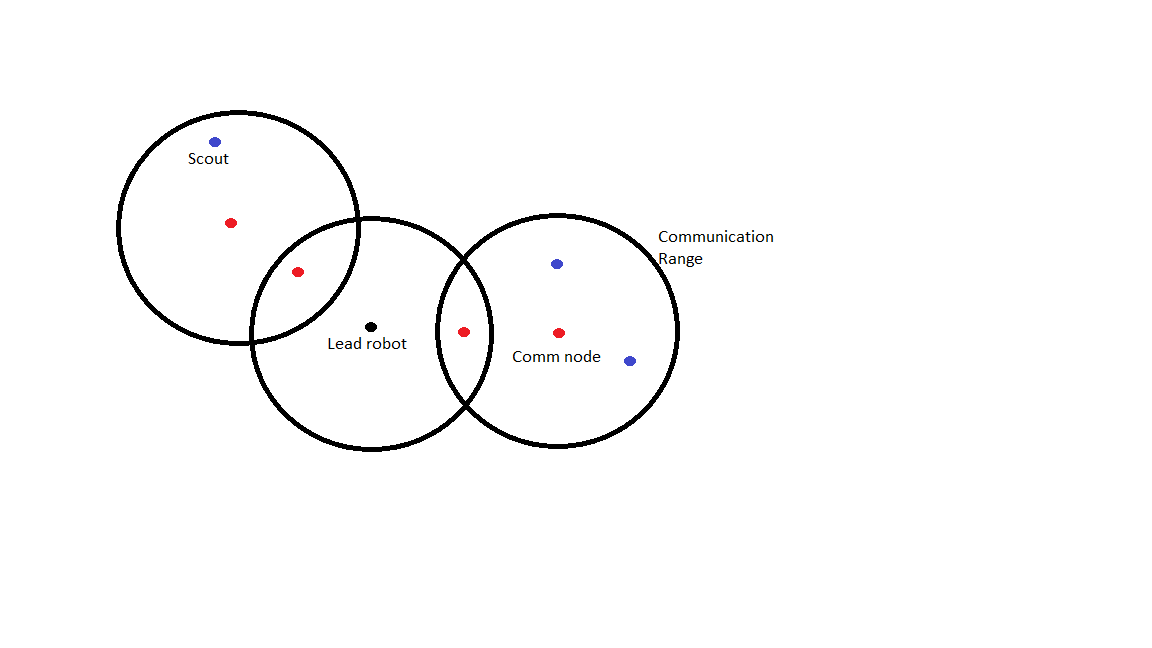
\includegraphics[width = 0.8\textwidth]{../../figures/comm_example.png} 
\caption{An example of the communication link}
\label{Figure 1}
\end{figure}

Figure 1 shows one possible example of the communication link, where the lead robot/ or in some cases a stationary uplink point is in the center and the communication robots(in red) placed in such positions that their comm range overlaps the comm range of other robots and the lead robot. \\
This configuration allows the scouts(in blue) to move and explore anything inside the communication range of the different comm robots. When the robots at the right side of the figure would now try to move outside the comm range one of them would have to change their behaviour pattern to "communication mode" at the outer range of the other comm nodes range while the last remaining scout continuous exploring in this direction. \\
This example shows that it is important to have a swarm of a suitable size for an environment to be able to cover at much area with the robots at hand and for cases in which this is not possible to be able to move the whole swarm in one unified direction to explore unmapped locations. This is however only doable when there is a lead robot since a stationary comm/uplink point is by definition, stationary.\\

\section{Analysis}
Taking into account the problem and what you learned from the background work, what was your analysis of the problem? How did your analysis help to decompose the problem into the main tasks that you would undertake? Were there alternative approaches? Why did you choose one approach compared to the alternatives? 

There should be a clear statement of the objectives of the work, which you will evaluate at the end of the work. 

In most cases, the agreed objectives or requirements will be the result of a compromise between what would ideally have been produced and what was felt to be possible in the time available. A discussion of the process of arriving at the final list is usually appropriate.

\section{Process}
You need to describe briefly the life cycle model or research method that you used. You do not need to write about all of the different process models that you are aware of. Focus on the process model that you have used. It is possible that you needed to adapt an existing process model to suit your project; clearly identify what you used and how you adapted it for your needs.


%\addcontentsline{toc}{chapter}{Development Process}
\chapter{Design}

This section will describe the design as of the date of the project outline description. \\
This is the design which will be followed and tried to implement, however this is more of a guideline rather than exact plan since at this moment it is uncertain what the  API and simulator are able to do and what is possible to implement inside the given time.\\

\section{Environment Design}
The final environment for this project will consist of one large room with obstacles placed in it. \\
The program will be tested on a number of different sized rooms with different amount and sized obstacles in it.


\begin{figure}[h]
\centering
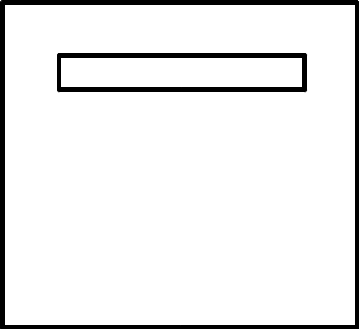
\includegraphics[width=0.5\textwidth]{../../figures/environment_example2.png} 
\caption{Environment Design}
\label{Figure 2}
\end{figure}

\section{Mapping and Swarm Size}
For mapping I will use a occupancy grid, and the occupancy will be acquired by the E-Puck's laser sensors. 
I will yet have to decide on a resolution, for the grid.\\
I will use a swarm of 5 E-Puck robots, of which 1 will remain stationary and only function as the "Uplink point" to which all robot send the acquired data. 
The stationary robot will also be used as reference point for the localisation method.

\section{Deployment}
It is at this moment still undecided which deployment strategy will be implemented. \\
There are 2 deployment strategies which are based on the background research which has been done.\\[3ex]

\subsection{Considered Deployment algorithms}

One which is based on a random walk though the environment which will turn to a random heading when an obstacle has been reached. \\
This approach could be combined with a wall following algorithm which would trigger a random walk when the same position is reached again. This would allow for the complete traverse of a obstacle/wall. This would require a good localisation solution as without it the robot will be stuck inside an eternal loop.\\[3ex]

The other deployment strategy would implement a more controlled movement pattern. This pattern would move the robots inside a rectangular pattern which would implement a function to move around obstacles on the way before moving back into the original pattern. 
While this reason is more controlled I am not sure which one will turn out to be more effective, that it why I will implement both inside a testing phase and will then decide which of them I will use.

\begin{figure}[h]
\centering
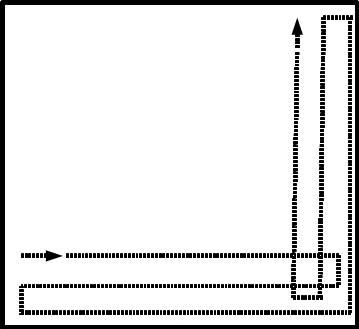
\includegraphics[width=0.5\textwidth]{../../figures/movement_pattern.png} 
\caption{Controlled movement Pattern}
\label{Figure 3}
\end{figure}

\subsection{Adopted design}
It was decided to adopt and implement the more controlled movement pattern which can be seen in figure \ref{Figure 3}.
dasdasdasd


\chapter{Implementation}
\label{Implementation}

\section{Early Development}
After the first weeks where background reading were done and designing a plan for the final program, work using the Webots\textsuperscript{\texttrademark} simulator was started. \\ More information about the different stages can be found in the following sub-sections. 

\subsection{Webots Tutorials}
In the beginning different tutorials and demo following  programs included in the Webots installation were followed. 
This helped to see how the simulator works, what it can do and what possibilities the Webots API gives an developer. \\
The tutorials used were provided by the Webots wikibooks site \footnote{\url{http://en.wikibooks.org/wiki/Cyberbotics\%27_Robot_Curriculum}}.\\
Starting off with simple tutorials and movement and sensor reading the developer was soon able to implement simple programs which were based on simple forwards movement with obstacle avoidance functions, based on the proximity sensor values. 
After some of the more "advanced"(in comparison to what had been done to this point) tutorials which involved e.g.: reading the robot encoders look at example programs of more advanced types of movement as well as SLAM examples were taken. \\

\subsection{First Program Iterations}
After that the experience of the tutorials was taken and it was started on to actually implementation the first prototype of the program. \\
The first prototype was still heavily based on a Webots example program called "Intermediate Lawn Mower" which involved a simple movement pattern based on a basic finite state machine(FSM). \\ 
The first attempt was based recreating the FSM to get the same basic movement capabilities as the the program it was based upon and than changing it to achieve the level of movement control which was needed. \\[3ex]

In the following iteration it was tried to implement the functionality of moving a given distance based on resetting the stepper motors encoders and moving the robot until it reaches a given encoder value. It was quickly realised that this would not work with the way the FSM was currently implemented so it was decided to move the functionality of the FSM, which was currently based on a simple switch statement, to a set of separate functions. The idea was that this would give the freedom needed to be able to call a method, i.e. \textit{move\_forward()},  and keep it running until a predefined encoder value has been reached. \\
However this did not work based on the overall way the program was designed at this point. It was designed around an switch statement which based its decisions on the proximity sensors of the E-Puck and then setting the movement speed for the robot motors. As it was based on this calling separate functions to move and turn did not work, which resolved in problems around the current idea of using the stepper motor encoders. \\[3ex] 

As it was needed to be able to move a certain distance in order to effectively implement the rectangular movement pattern, various approaches which were all based around the FSM were tried. 
It was realised soon that this was not getting anywhere which this way of thinking so it decided to come back to this problem later and went to another problem: turning a given number of degrees. \\
As the simulator simulates friction between the robot wheels and the environment the turning function, as it was in it current state, was far to inaccurate to be usable. \\
It was based on a very basic odometry calculation, taking the encoder values and calculating the turning distance based on the wheel diameter and axle length of the robot. While this is not a bad approach it had no procedures of slowing down the movement as it got closer to the target state so overshooting the wanted position or rotating far to less if the motor speed would have been set to low. \\
It was tried to counter the problem by alternating the values it used for the odometry calculations, and while it came close to a solution it was far from accurate. Another problem with this solution was that it only worked for ~90 degree rotations based on the modified values, meaning all rotations to another point were impossible without modifying the values to fit the target heading. Which was counter productive as it would be best to have 1 function able to orientate the robot to any wanted heading. \\

\section{Mid stage Development}
After the problems which were encountered during the first program iterations, it quickly realised that this way of thinking and understanding of the API was flawed. A lot of the problems which were encountered were the result of insufficient programming skills for what  was tried to do combined with bad understanding of how odometry worked, and how this could be used it to control the robot.\\
Seeing these kinds of problems it was decided to take a step back as the thought process for the program design was clearly "moving in circles" and encountering the same kind of problems over and over again with the current approach. \\
It was decided to take once more a look at the provided example programs and to study their odometry functions in order to gain some new insight into odometry calculations, and find a new approach based on that.

\subsection{Advanced tutorials}
The example programs provided together with the simulator are categorised after the estimate level of knowledge needed to complete them. Theses categories are: Beginner, Novice, Intermediate and Advanced. The advanced programs were already looked at before as they feature a couple of examples on odometry and slam, however they were not understood  well enough at the time.\\ 
Looking closer at the odometry functions provided it was managed to understand a bit better how the advanced programs worked and how they calculated the movement of the robot. \\[3ex]

A look was also taken at the code and notes which were taken during the Robotics module on the second year, while the API worked different for the Player/Stage environment the idea behind rotation and movement was still the same and had only to be applied using the Webots API.

\section{Movement}
After having studied the odometry functions of the provided programs it was decided to start a new approach to fix the movement of the robot.\\
This approach is based on a set of different functions, much smaller and more refined than my previous approach. This approach took a while to implement and test but the results were rather satisfactory. This section is going to describe the different aspects of the movement solution and describe how the most important functions work.\\
The code of the major functions will be added as appendices, the site numbers will be added to each subsection. It is worth noting that the code displayed in the appendix is the final version of the code, and often updated in comparison to what they are at this stage in the development process. 

\subsection{Moving Forward}
\label{moving_forward_description}
The code for this function can be found in Appendix B, section \ref{moving_forward_code} at page \pageref{moving_forward_code}.\\
It is worth noting at that the code display in appendix B is the final version, the earlier versions of this code did not hold the odometry update function \textit{odometry\_track\_step()}.
The \textit{move\_forward }function takes 2 doubles as parameters, 1 being the speed with which the robot is ordered to move and the distance it should move. The last parameter is a link to the global odometry struct, this struct is used to update the odometry values.\\
The function first checks that neither of the parameters are 0 and then calculates the number of steps each motor has to drive(1 step being 1 step of the stepper motor) to reach its target position.
This calculation is done by dividing the number of steps needed for a full wheel rotation, 1000 in this case, by the product of $\pi$ times the wheel diameter times 2 and multiplication this result with the distance defined in the parameter of the function. The steps needed for a full rotation have been taken from the E-Puck documentation and have been confirmed during on of the odometry tutorials. \\
It will then read the current encoder positions and calculate the stop position for each motor by the sum of the encoder values for each motor and the previously calculated encoder steps needed to reach the target area. 
It will then set the motor speed based on the speed defined in the parameters.\\[3ex]

It then enters the control code which will stop the robot once it reaches it target, position. \\
This is controlled by comparing the current encoder positions with the calculated target encoder positions and updating them all the time. 
Once the robot reached a pre-defined minimum distance of 20 encoder steps it will slow down the movement to a minimum speed of 10 steps per second. This is down to prevent the robot from overshooting the target area should it move with to much speed. The optimal minimum distance and speed has been found experimentally, and both values give good results and also prevent the robot from undershooting.
Once it has reached it target location it will stop the robot, and force the simulator to take a simulation step, effectively moving onward to the next command.\\[3ex]

This function allows the robot to move forward and stop after the predefined distance within a minimal error space, which will always exist given the friction simulated inside the simulator. This method required a lot of testing in order to get right as first versions did not include the control statement which slowed down the robot after a minimum difference between the encoders and the target encoder value has been reached. So the robot used to overshoot the target. \\
After the control statement was implemented it still required some testing and calibration of the minimum difference and speed values in order to avoid over and undershooting. However the found values work well and the movement error has been reduced to minimum.\\

\subsection{Turn a given angle}
\label{turn_angle_description}
The code for this function can be found in Appendix B, section \ref{turning_angle_code} at page \pageref{turning_angle_code}.\\
The turn\_angle function takes 2 doubles as parameters, one being the angle the robot will turn to the other the speed with which the robot will turn.\\
First the factor by which the robot will turn is calculated by dividing 360, the value of a full rotation, with the defined angle.
Once the factor has been calculated it will then the number of steps the motor have to do until the target position is reached. This is done by dividing the product of the steps needed for a full wheel rotation, 1000, and the size of the wheelbase by the product of the calculated turning factor and 2 times the wheel radius. It will then use a function to return the current motor encoder positions. This function simply uses the Webots\textsuperscript{\texttrademark}  API and returns the values. \\[3ex]

If the rotation angle defined as the function parameter is positive the robot will turn to the right.\\
When the robot is turning to the right it will calculated the stopping positions of the encoders by adding the calculated step count to the left motor encoder and subtracting it from the right encoder. This will lead to the wheels turning against each other and will result in the robot turning on the spot rather than only moving 1 wheel to turn which would result in a displacement of the robot. \\
And then set the the speed of the motors using the given function parameter value. The right motor will receive a negated value so that it will turn backwards. 
It will then compare the left encoder positions and updated them all the time. Similar to how the forward movement function worked, it will detect when a given minimum difference between the current and target encoder values is reached and slow the robot down to a minimum speed. \\[3ex]

If the rotation angle defined as the function parameter is negative the robot will turn to the left.\\
The only difference between turning left rather than to the right is that the calculations, obviously, are reversed. Meaning to calculated the stop positions of the motor encoders it will subtract the calculated step count from the current left encoder value and add the step count the the right
encoder value, same switch of negation has been done where the motor speeds are set.
The calculations of how long to turn and when to slow down are identical to how they work when turning right, only difference being that the the operators to which check how long to turn are different.\\
Once the target position has been reached, by either turning left or right, the robot stops.
It will then force to the simulator to take a simulator step, effectively moving on to the next command.\\[3ex]

This functions allows me to define the turn the robot by so many degrees as I need and it will turn there within an minimal error space. This error space exist because the simulator simulates friction between the robot wheels and the environment so 100\% accurate movement will never happen.\\
There also existed the problem of over/undershooting with the turning however the values found during tests of the \textit{move\_forward} function turned out to also work well for the turning function. However one problem remains, since there never is going to be a perfect rotation the error value will add up over time, resulting in less and less accurate turns, overshooting the target rotation is going to be a real problem. I have at this point not yet a solution for this problem, however the function works well and is a great improvement to how it turning was implemented in previous iterations of the program.

\section{Localisation using Odometry}
After the studying the optometry functions provided and implementing the movement algorithms, it was time to implement the localisation using odometry calculations.\\
The odometry functions which were implemented are used for localisation the robot inside the environment and finding it heading. The functions only require the starting point and localisation of the robot, and are then able to calculate the movement and rotation of the robot with every movement done, within a certain degree of accuracy. The uncertainty in accuracy is based on the friction which get simulated inside the simulator. \\
These functions are largely similar to the ones provided with the Webots\textsuperscript{\texttrademark} interface, however some minor changes has been done. \\
Similar to the way in which the movement algorithms have been described the odometry functions are going to be described. 

\subsection{Initialising the Odometry algorithms}
\label{odometry_init_description}
The code for this function can be found in Appendix B, section \ref{odometry_init_code} at page \pageref{odometry_init_code}.\\
The code for the odometry struct can be found in Appendix B, section \ref{odometry_struct_code} at page \pageref{odometry_struct_code}.\\
To initialize the odometry algorithms, 2 functions are used. \\
The first function, \textit{odometry\_track\_start} takes a \textit{odometrtyTrackStruct}, which is defined in the class which calls the function, as parameter. It will then acquire the encoder positions of the robot and call the next function, \textit{odometry\_track\_start\_pos} which set's the starting values, including the encoder positions inside the odometry struct.\\[3ex]


Also the distance travel when a wheel turns and the wheel conversion are calculated, used for this are parameters acquired during calibrations done in the Webots \textsuperscript{\texttrademark} example programs(the values are the same as it is the same virtual robot model) and the E-Puck documentation. 

\subsection{Updating the Odometry values}
\label{odometry_update_description}
The code for this function can be found in Appendix B, section \ref{odometry_update_code} at page \pageref{odometry_update_code}.\\
To update the odometry values of the struct the function \textit{odometry\_track\_step} is called.
When this function is called inside another function a number of things happen.\\
The current encoder positions for the stepper motors are fetched, 
and used as a parameter inside the \textit{odometry\_track\_step\_pos} function call. \\
Inside this function the new X, Y coordinates and the rotation of the robot are calculated. This is achieved by first calculating the difference between the current encoder positions and the encoder previous encoder positions saved inside the struct. 
This difference is then multiplied by the wheel conversion, which gets calculated inside the initialization step. \\
The result of this is used to calculated the wheel movement of the left and right wheel, results which are used to calculate the rotation of the robot. 
The next step is to calculate the new X and Y coordinates of the robot, based on the sum of done left and right wheel movement  and math calculations using the robots rotation. 
At the end the calculated X and Y coordinates as well as the rotation value are used to update to struct. And the current encoder positions are saved inside the buffer for later calculations. 

\subsection{Minimum speed and distance calibration}
\label{mov_calibration}
After these functions were created they were calibrated using following processes .\\

\begin{figure}[h]
\centering
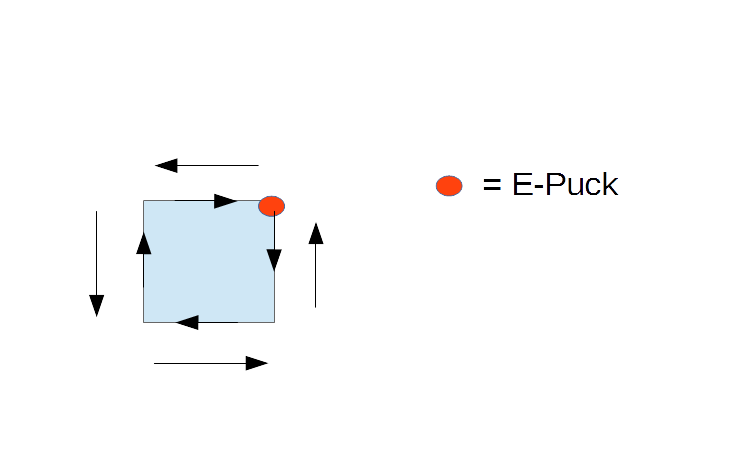
\includegraphics[width = 0.5\textwidth]{../../figures/movement_test.png} 
\caption{Movement algorithm test pattern}
\label{movement_test}
\end{figure}

Figure \ref{movement_test} shows a simple movement pattern which was used to calibrate the minimum turn distances and tested that the \textit{move\_forward()} and \textit{turn\_angle()} methods worked as intended. \\
How it works is the E-Puck starts on 1 corner of a square(here the floor of the simulator was used as it has chessboard representation) and move forwards to the other end of the square, turn 90 degrees and so on until it reaches it start point. It then turns around and follows the same pattern back to its original starting position. This tests allows the notice of odometry error in the rotations and forward movement, after a while it would turn/move to far or not far enough and thereby not reach it accurate start point. Noticing these errors allowed for calibration of the speed and distance where the algorithms will slow done the movement to minimize this error as much as possible, see section \ref{moving_forward_description} and \ref{turn_angle_description} respectively for more information on this.\\[3ex]
The test is based on the "University of Michigan Benchmark" or UMBmark\footnote{\url{http://www.cs.columbia.edu/~allen/F13/NOTES/borenstein.pdf}}.\\[3ex]

The problem with this calibration at the time was rather than using this approach to calibrate the effective wheelbase and the wheel radius at the time of this calibration the angles to turn were changed.\\
This led to rather than updating the wheelbase from  the original 0.052(which has been done in a later stage of the project. \textbf{Note: the code which can be found in Appendix B uses the updated wheelbase}.\\
Using the non-updated wheelbase it was required to change specify an angle of 100$^{\circ}$ to move 90$^{\circ}$ effectively.

\section{First results}
After the calibration process of the previous section a new program iteration was started, using the new movement and localisation algorithm in order to test the mapping and continue implementing it. \\[3ex]

This first implementation was not using the deployment pattern but rather simply following the walls, this was done so that the mapping could be tested. Rather than having an advanced wall following algorithm at this stage a simple collision avoidance algorithm was used which turned the robot by 90$^\circ$ when ever an obstacle is reached. 

\subsection{Early mapping methods and results}

\begin{lstlisting}[caption={Proximity sensor reading}]
//distance sensors array definitions
int ps_value[NUM_DIST_SENS]={0,0,0,0,0,0,0,0};
int obstacle[NUM_DIST_SENS]={0,0,0,0,0,0,0,0};
int ps_offset[NUM_DIST_SENS] = {35,35,35,35,35,35,35,35};

// obstacle will contain a boolean information about a collision
for(i=0;i<NUM_DIST_SENS;i++){
	ps_value[i] = (int)wb_distance_sensor_get_value(ps[i]);
	obstacle[i] = ps_value[i] - ps_offset[i] > THRESHOLD_DIST;
}

//define boolean for sensor states for cleaner implementation
bool ob_front =
	obstacle[PS_RIGHT_10] ||
	obstacle[PS_LEFT_10];

bool ob_right =
	obstacle[PS_RIGHT_90];

bool ob_left =
	obstacle[PS_LEFT_90];
\end{lstlisting}

The code above shows the code used at this stage of the project to detect obstacles, and set boolean values if an obstacle is detected in the direction of the  obstacle. As the test environment for this part of the project is a simple square area the turning of 90$^{\circ}$ is sufficient and no other control was needed at this stage to test the mapping. 

\begin{figure}[h]
\centering
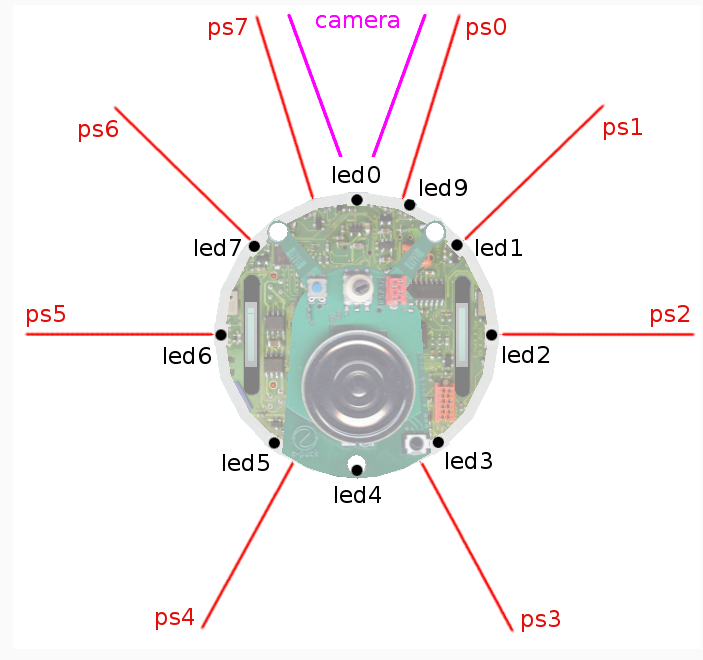
\includegraphics[width = 0.5\textwidth]{../../figures/e_puck_sensor_placement.png} 
\caption[E-Puck sensor placement]{E-Puck sensor placement\footnotemark}
\label{sensor_placement}
\end{figure}

Figure\footnotetext{Figure \ref{sensor_placement} is taken from: \url{http://www.cyberbotics.com/cdrom/common/doc/webots/guide/section8.1.html}}  \ref{sensor_placement} show the sensor placement on the E-Puck robot. Its is worth noticing that for sake of simplicity and better work flow the sensors have been renamed in the code. The new naming scheme does show which side of the robot the sensor is placed and its placement in degrees, relevant to the forward facing center of the robot. As an example the sensor ps0 in figure \ref{sensor_placement} is named PS\_RIGHT\_10 in the code since it is placed on the right side of the robot with an orientation of 10$^{\circ}$ relevant to the center.
Compared to this sensor ps5 is PS\_LEFT\_90.   \\[3ex]

The mapping algorithm used a similar approach to the obstacle detection algorithm. \\
One of the problems which were noticed at this stage was the problem of the noise simulated inside the simulator, this leads to the mapping algorithm needing a high threshold in order to map only actual obstacles, and not random noise spikes.  This however leads to the problem of the robot needing to almost be in direct contact with the obstacles in order to map them. For the mapping at this stage this was not a problem however this strongly influenced movement pattern decisions at a later stage in the implementation process, more about that in a later section.

\begin{figure}[h]
\centering
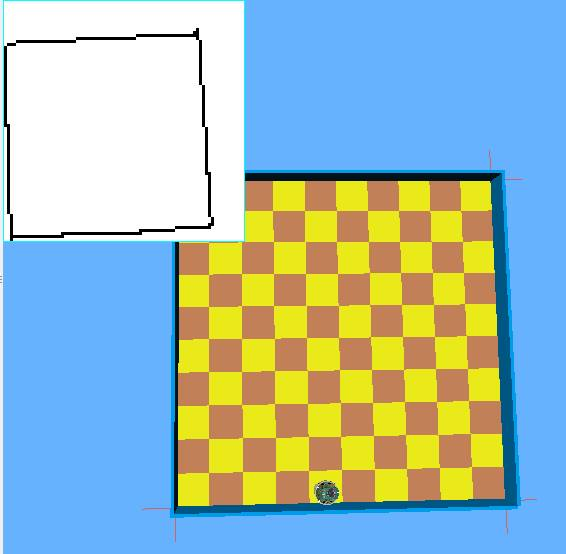
\includegraphics[width = 0.5\textwidth]{../../figures/early_map.jpg} 
\caption{Early mapping result}
\label{early_mapping_result}
\end{figure}

Figure \ref{early_mapping_result} shows clearly the strongest problems with this solution so far as well as demonstrates the need to have a good solution for  the main aspects of this project, localisation and deployment.\\
As it can clearly be seen in the figure, the localisation and movement approach were far from perfect at this stage in the project. 
While the program generates a closed  map the mapping is strongly skewed to the left side. This error was strongly based on odometry errors during turning caused by sup-optimal calibrated robot values as well as friction between the wheels and the floor.\\
At the time to movement algorithm did not update the odometry struct, and the struct were only updated once every loop iteration. \\
This was the stage of the project at the time of the mid-project demo.


\subsection{Direction control based on heading}
The approach done to fix the odometry error at this stage was done by specifying directions in which the robot is moving as north, east, south and west. 

\begin{figure}[h]
\centering
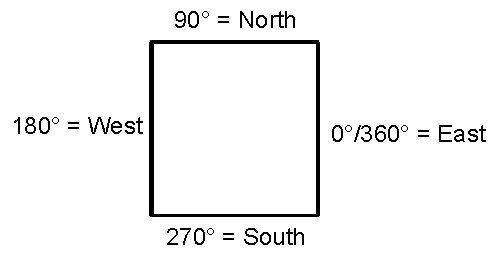
\includegraphics[width = 0.5\textwidth]{../../figures/direction_and_angles} 
\caption{Directions and their corresponding Angles}
\label{directions_and_angles}
\end{figure}

Figure \ref{directions_and_angles} does show the directions used and the corresponding angles. The directions were represented in the code by using boolean values. \\
In order to get the direction controlled movement working a number of functions needed to be created.  

\begin{lstlisting}[caption={Converting Radians to degrees}]

#ifndef M_PI
	#define M_PI 3.1415926535897932384626433832795L
#endif

#define RTOD(r) ((r) * 180 / M_PI)

/**
returns the angle in which the robot is moving
*/
int return_angle(double rad){
	double rotation;

	if(RTOD(rad) < 0){
		rotation = RTOD(rad) + 360;
	}else{
		rotation = RTOD(rad);
	}
	printf("%f\n", rotation);
	return rotation;
}
\end{lstlisting}

This function converts radians, which are used by the simulator, to degrees.This was done to make it easier to work with.
The next function uses this to check in which direction the robot is moving and set a boolean value representing a direction to \textit{true}.

\begin{lstlisting}[caption={Early check of the movement direction}]
#define ANGLE_TOLERANCE 20
#define EAST 0
#define NORTH 90
#define WEST 180
#define SOUTH 270

//direction definitions
bool north,west,south,east;

/**
set booleans for the direction the robot is moving in
*/
void check_direction(double d){
	int i = return_angle(d);
	east = false;
	north = false;
	west = false;
	south = false;

	if(EAST < i + ANGLE_TOLERANCE || EAST > i - ANGLE_TOLERANCE){
		east = true;
	}else if(NORTH < i + ANGLE_TOLERANCE || NORTH > i - ANGLE_TOLERANCE){
		north = true;
	}else if(WEST < i + ANGLE_TOLERANCE || WEST > i - ANGLE_TOLERANCE){
		west = true;
	}else if(SOUTH < i + ANGLE_TOLERANCE || SOUTH > i - ANGLE_TOLERANCE){
		south = true;
	}
}
\end{lstlisting}

At this moment the deployment pattern described in chapter \ref{Design}  was also implemented. \\
This was done by checking which direction the robot is facing when an obstacle is found in front of the robot. At this point a couple of procedures were designed for what to do for each direction. Effectively the robot is performing u-turns when ever an obstacle is found directly in front of it. 

\begin{figure}[h]
\centering
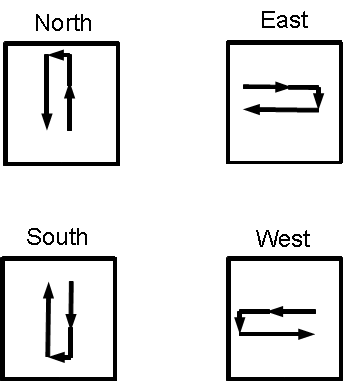
\includegraphics[width = 0.5\textwidth]{../../figures/direction_uturn_pattern} 
\caption{Directions and their corresponding U-Turn pattern}
\label{directions_uturn_pattern}
\end{figure}

The u-turn patterns shown in figure \ref{directions_uturn_pattern} effectively led the robot to move from right to left and from the top downward, there wasn't any particular reason for this, other than an uniformed pattern was needed. \\ 
The next piece of code is a snipped from the deployment loop at that time in the project. It uses the previous shown \textit{check\_direction()} as well as the \textit{controll\_angle()} method which will be shown at a later point.\\
The control angle function is used to compare the current heading with the heading specified by the general direction the robot is moving in(north/east/south/west). 
As the code snipped shows at this point the the odometry struct is still not updated during the deployment loop, and the heading is only checked and corrected in the FORWARD state of the loop. 
The \textit{turn\_right()} and \textit{turn\_left()} functions turn the robot 90$^{\circ}$.

\begin{lstlisting}[caption={Early Control loop snipped}]
double dMovSpeed = 500.0f;
double dDistance = 0.01f;
double dTurnSpeed = 100.0f;
double dTurnDistance = 0.05f;	

switch(state){
	case FORWARD:
		move_forward(dMovSpeed, dDistance);
		controll_angle(&ot);
		if(ob_front){
			state = STOP;
		}
		break;	
	case STOP:
		stop_robot();

		if(ob_front && ob_left){
			state = TURNRIGHT;
		}
		else if(ob_front && ob_right){
			state = TURNLEFT;
		}
	else if(ob_front){
		check_direction(ot->result.theta);
		state = TURNRIGHT;
	}
	break;	

	case TURNRIGHT:
		turn_right(dTurnSpeed);
		state = FORWARD;
		break;
	case TURNLEFT:
		turn_left(dTurnSpeed);
		state = FORWARD;
		break;
	case UTURN:
		if(north){
			turn_left(dTurnSpeed);
			move_forward(dTurnSpeed, dTurnDistance);
			turn_left(dTurnSpeed);
			state = FORWARD;
		}else if(south){
			turn_right(dTurnSpeed);
			move_forward(dTurnSpeed, dTurnDistance);
			turn_right(dTurnSpeed);
			state = FORWARD;
		}else if(west){
			turn_left(dTurnSpeed);
			move_forward(dTurnSpeed, dTurnDistance);
			turn_left(dTurnSpeed);
			state = FORWARD;
		}else if(east){
			turn_right(dTurnSpeed);
			move_forward(dTurnSpeed, dTurnDistance);
			turn_right(dTurnSpeed);
			state = FORWARD;
		}
		east = false;
		north = false;
		south = false;
		west = false;
		break;
	default:
		state = FORWARD;
}
\end{lstlisting}

It is worth mentioning that this approach went through a number of modifications before this state was reached. The previous modifications were done to check to optimal placement of the \textit{controll\_angle()} function. It was found to be unproductive to have the check after every turn, as it did not matter on the small distances the robot was moving in the u-turn process. \\

\begin{lstlisting}[caption={Early heading correction algorithm}, label={early_heading}]
 /**
Controll the movement angle
*/
void controll_angle(struct odometryTrackStruct *ot){
	int rotation;
	int dSpeed = 100.0f;
	int corAngle = 5.0f;

	if(RTOD(ot->result.theta) < 0){
		rotation = RTOD(ot->result.theta) + 360;
	}else{
		rotation = RTOD(ot->result.theta);
	}

	//check movement to the right(east)
	if(EAST < rotation + ANGLE_TOLERANCE){
		turn_angle(-corAngle, dSpeed);
	}else if(EAST > rotation - ANGLE_TOLERANCE){
		turn_angle(corAngle, dSpeed);
	}

	//check movement to the north
	if(NORTH < rotation + ANGLE_TOLERANCE){
		turn_angle(-corAngle, dSpeed);
	}else if(NORTH > rotation - ANGLE_TOLERANCE){
		turn_angle(corAngle, dSpeed);
	}

	//movement to the west
	if(WEST < rotation + ANGLE_TOLERANCE){
		turn_angle(-corAngle, dSpeed);
	}else if(WEST > rotation - ANGLE_TOLERANCE){
		turn_angle(corAngle, dSpeed);
	}

	//movement to the south
	if(SOUTH < rotation + ANGLE_TOLERANCE){
		turn_angle(-corAngle, dSpeed);
	}else if(SOUTH > rotation - ANGLE_TOLERANCE){
		turn_angle(corAngle, dSpeed);
	}
}
\end{lstlisting}
The code above is an early version of the algorithm which checks and corrects the heading the robot is moving in. This algorithm was used to correct the odometry error caused by the friction in the environment and the, at this stage, sub-optimal calibrated robot attributes. \\
It worked by comparing the heading the robot is heading in with the wanted heading and correcting any errors. The algorithm at this stage has some short comings such as it is not possible to turn the robot more accurate than with a 5$^{\circ}$ threshold. If the threshold was reduced to less than  5$^{\circ}$, the robot would constantly overturn. \\[3ex]

At this time it was assumed that this inaccuracy was caused by the friction simulated inside the simulator, and that this movement was as accurate as it was going to be. \\
The odometry error at this stage did improve thanks to the \textit{control\_angle()} functions, the start of the mapping was much less skewed than the previous approach, which result can be seen in function \ref{early_mapping_result} at page \pageref{early_mapping_result}. \\[3ex]

However the constant odometry error did accumulated over time, so that the location displacement became to big to able to map the environment effectively. \\
In order to try to fix the localisation error, a couple of approaches were done in order to reduce said error. Before those approaches were done some refactoring and code improvement was done.

\section{Refactoring and improvement}
In this section the refactoring and code improvements which were done at this stage of the project is described. \\
Some of the refactorings I have not addressed in this section are the movement of functions to other source files.
While it clearly is good practise to create functions at the right place in the first place, a lot of prototype functions were created in the main source files for sake of simplicity during the first functions test. These functions were later moved to other source files were they are more appropriate, and to keep the overall source file size done. 

\subsection{Deployment algorithm refactoring}
Before other approaches were tried it was decided that the deployment algorithm needed to refactored to make the code cleaner and easier. \\
The following piece of code is a snipped taken from one of the algorithm:

\begin{lstlisting}[caption={Deployment algorithm refactoring}]
double dSpeed = 500.0f;
double dDistance = 0.01f;

char no[] = "north";
char ea[] = "east";
char we[] = "west";
char so[] = "south";

case UTURN:
	if(north){
		printf("%s\n", no);
		turn_left(dTurnSpeed);
		for(it = 0;it < 5;it++){
			move_forward(dSpeed, dDistance);
		}
		turn_left(dTurnSpeed);
		north = false;
		state = FORWARD;
	}else if(south)[...]
\end{lstlisting}

As the above snipped shows the unneeded variables of \textit{dTurnSpeed} and \textit{dTurnDistance} were removed as it was decided that the algorithm, for simplicities sake, use a single value type which can easily be changed. In order to get the same amount of movement during the u-turn phase a simple \textit{for loop} is used. The same modifications as are shown in the code snipped have been done to the rest of the u-turn \textit{case}. \\
In order to improve the code further, printout statements were added to the u-turn routine as well as to the \textit{return\_angle()} function.
This needed to be done as the webots simulator does not have a debugger, so printouts were used to track to results of the algorithms.

\subsection{Deployment algorithm improvement}
\label{deployment_improvement}
The previous u-turn method did not support mapping obstacles while the u-turn was performed. As this is not optimal behavior the u-turn pattern was altered again, to support the mapping methods. 

\begin{lstlisting}[caption={U-turn improved with obstacle detection and mapping}, label={uturn_code}]
#define NUM_DIST_SENS 8 //number of distance sensors 
#define OCCUPANCE_DIST 150 //obstacle mapping threshold
double dSpeed = 500.0f;
double dDistance = 0.01f;

static int wtom(float x){
	return (int)(MAP_SIZE / 2 + x / CELL_SIZE);
}

robot_x = wtom(ot->result.x);
robot_y = wtom(ot->result.y);

char no[] = "north";
char ea[] = "east";
char we[] = "west";
char so[] = "south";

case UTURN:
	if(north){
		printf("%s\n", no);
		turn_left(dSpeed);
		for(it = 0;it < 5;it++){
			move_forward(dSpeed, dDistance);
			
			//mark cells as occupied
			wb_display_image_paste(display,background,0,0);
			wb_display_set_color(display,0x000000);
			for(i = 0;i < NUM_DIST_SENS;i++){
				if(wb_distance_sensor_get_value(ps[i]) > OCCUPANCE_DIST){
					occupied_cell(robot_x, robot_y, ot->result.theta + angle_offset[i]);
				}
			}
			wb_display_image_delete(display,background);
			background = wb_display_image_copy(display,
				0,0,display_width,display_height); 
		}
		turn_left(dSpeed);
		north = false;
		state = FORWARD;
	}else if(south){[...]
\end{lstlisting}

The above code shows how the obstacle detection and mapping were added to the u-turn \textit{case}. 
This map's the obstacles to the sides of the E-Puck while the robot moves along the side of it and proceeds to the next turn. While this mapping is not good, as it is very "spotty".

\begin{figure}[h]
\centering
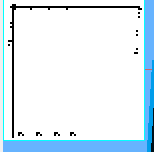
\includegraphics[width = 0.5\textwidth]{../../figures/map_results/dotted_uturn_mapping.png} 
\caption{Dotted mapping during U-Turns}
\label{dotted_uturn}
\end{figure}

Figure \ref{dotted_uturn} shows the dotted mapping which is caused during u-turns. While it is in no form a good representation of the environment it provides an outline of obstacles. The problem with this is however that because of the u-turn pattern it is needed for the robot to traverse a long each obstacle / wall in order to map them correctly. 

\section{Mapping}
In this section the mapping algorithm are shown and described. \\
The mapping algorithms are one of the key algorithms of the project, however based on code from the Webots\textsuperscript{\texttrademark} demo programs It is based on a occupancy map, which is a simple 2D map. The function used to mark a \textit{cell} of the occupancy map.\\
The code for this function can be found in Appendix A, section \ref{occupied_cell} on page \pageref{occupied_cell}.
The parameters for the function represent the X and Y coordinates as well as the rotation of the robot. These values are received from the odometry struct. 
The functions uses the Webots\textsuperscript{\texttrademark}  API to draw the cell in form of a 1x1 pixel rectangle on the display. 

\begin{lstlisting}[caption={obstacle detection and mapping}]
#define NUM_DIST_SENS 8 //number of distance sensors 
#define OCCUPANCE_DIST 150 //obstacle mapping threshold

static int wtom(float x){
	return (int)(MAP_SIZE / 2 + x / CELL_SIZE);
}


robot_x = wtom(ot->result.x);
robot_y = wtom(ot->result.y);

wb_display_image_paste(display,background,0,0);
wb_display_set_color(display,0x000000);
for(i = 0;i < NUM_DIST_SENS;i++){
	if(wb_distance_sensor_get_value(ps[i]) > OCCUPANCE_DIST){
		occupied_cell(robot_x, robot_y, ot->result.theta + angle_offset[i]);
	}
}
wb_display_image_delete(display,background);
background = wb_display_image_copy(display,0,0,display_width,display_height); 
\end{lstlisting}

The code above shows for loop which checks the value reported by each 1 of the 8 distance sensors and compare this value to the defined threshold. If the value is larger than the threshold the cell will be marked. 

\section{Refactoring of the heading correction}
In this section the refactoring of the heading correction functions is shown. 
The earlier version of this code can be seen in listing \ref{early_heading} on page \pageref{early_heading}.
The earlier version of this code snipped worked, however it was way more complex than it had to be. 

\begin{lstlisting}[caption={Refactored heading control code} ]
/**
Function to compare the current heading to the wanted heading
and fix the heading should it surpass a threshold
*/
void check_rotation(double cur_rot, double want_rot, double dSpeed){
	double dthreshold = 1; //2,0
	double diff;
	char text[] = "Correcting";
	
	if(cur_rot + 20 >= 360){
		cur_rot -= 360; 
	} 
	
	if(cur_rot > want_rot + dthreshold){
		diff = cur_rot - want_rot;
		printf("%s\n", text);
		turn_angle(diff, dSpeed);
	}else if(cur_rot < want_rot - dthreshold){
		diff = want_rot - cur_rot;
		printf("%s\n", text);
		turn_angle(-diff, dSpeed);
	}
}
\end{lstlisting}

The newer version of this function only requires parameters with defines the wanted and the previous heading rather then the need of having global boolean values to specify in which direction the robot is moving. 
This refactored approach works by comparing the wanted and current heading, an threshold is also included as the robot will never turn 100\% accurate. \\
The function also converts degrees which are above 360 $^{\circ}$, to a more sensible value. 
The code holds printout statements which allow to understand in which direction the robot thinks it is moving, which can be compared to the actual direction for testing purposes. \\[3ex]

After this function was created the threshold was calibrated in a couple of runs. The threshold which was set in the first iteration, and was gradually decreased to a value of \textit{3} at the time. The threshold value shown in the code snipped above is \textit{1}, this value was reached by recalibrating the turning and movement functions, more about that can be found in section \textbf{FIXME(enter section number)}.

\section{New approach tried and implemented}
In this section the different approaches which were tried at this development stage are described. While not all approaches were successful not every aspect of them was discarded.

\subsection{Dynamic U-Turn approach}
At this point in the development process a new approach for turning the robot in the U-turn routine was tested. The idea was to change from using a static turning command \textit{turn\_left(dSpeed)}, which can be seen i code snipped \ref{uturn_code} on page \pageref{uturn_code}, to a more dynamic approach. \\
In this new dynamic approach the angle to turn was calculated from the current rotation and the wanted angle.

\begin{lstlisting}[caption={Code snipped of the new approach}, label={newApproach}]
double cur_rot;
	
else if(south){
	printf("%s\n", so);
	turn_right(dTurnSpeed);
	for(it = 0;it < 5;it++){
		move_forward(dTurnSpeed, dDistance);
		//mark cells as occupied
		wb_display_image_paste(display,background,0,0);
		wb_display_set_color(display,0x000000);
		for(i = 0;i < NUM_DIST_SENS;i++){
			if(wb_distance_sensor_get_value(ps[i]) > OCCUPANCE_DIST){
				occupied_cell(robot_x, robot_y, ot->result.theta + angle_offset[i]);
			}
		}
		wb_display_image_delete(display,background);
		background = wb_display_image_copy(display,0,0,display_width,display_height);
	}
	odometry_track_step(ot);
	cur_rot = return_angle(ot->result.theta);
	turn_angle(cur_rot - 90, dTurnSpeed);
	//turn_left(dSpeed);
	south = false;
	state = FORWARD;
}else if(west)[...]
\end{lstlisting}

The code in listing \ref{newApproach}, is a snipped from the U-turn routine. \\
However this approach did not work out as the robot always turned to far. Rather than getting stuck on this new approach, it was discarded and work was resumed with the old, static version of the code where the robot simply always turns 90$^{\circ}$. \\

\subsection{Stop on corner detection}
At this stage it was noticed that some of the existing odometry error existed because the robot did not stop when an obstacle, like a corner was encountered in the U-turn routine. 
What actually happened is that the robot wheels kept turning, increasing the encounter values, which let to wrong odometry calculations. \\
To fix this problem corner detection was added to the algorithm. 
It is worth noting at this point that rather than only corner detection, general obstacle detection should have been added. However, as it described in chapter 4, the program was only ever tested in the same environment during development which let to many of the problems encountered in the tests. 
The reason that only corner detection was added at this point was because it was known that the only obstacle which will be encountered in the U-turn routine are going to be corners, so no other type of obstacles was even considered.\\[3ex]

In the first iteration of this approach is corner detection was added \textbf{bellow} the section of code which mark's cells as occupied. Test runs quickly showed that it works better \textbf{before} said section, so the corner detection was moved.\\
The snipped shown in listing \ref{corner-uturn} is the final version with the corner detection above the cell marking section.

\begin{lstlisting}[caption={Corner detection added to the U-turn routine}, label={corner-uturn}]
if(north){
	printf("%s\n", no);
	turn_left(dSpeed);
	for(it = 0;it < 5;it++){
		if((ob_front && ob_right) || (ob_front && ob_left)){
			state = STOP;
			break;
		}
		move_forward(dSpeed, dDistance);

		//mark cells as occupied
		wb_display_image_paste(display,background,0,0);
		wb_display_set_color(display,0x000000);
		for(i = 0;i < NUM_DIST_SENS;i++){
			if(wb_distance_sensor_get_value(ps[i]) > OCCUPANCE_DIST){
				occupied_cell(robot_x, robot_y, ot->result.theta + angle_offset[i]);
			}
		}
		wb_display_image_delete(display,background);
		background = wb_display_image_copy(display,0,0,display_width,display_height); 
	}
	turn_left(dSpeed);
	north = false;
	state = FORWARD;
}else if(east){[...]
\end{lstlisting}

\subsection{Added odometry update function to the movement algorithm}
Until this stage the odometry values were only updated every control loop iteration. \\
In order to increase the number of odometry updates, which needed to be done in order to make the localisation more accurate, the odometry update function needed to be called more often then just once every iteration.
This was done in an approach to reduce the overall odometry error  by updating the \textit{odometry struct} more often, before odometry errors has a change to accumulate further. \\[3ex]

In order to implement this the odometry updated function was added to the \textit{move\_forward()} function. 
The code which can be found in Appendix B section \ref{moving_forward_code} on page \pageref{moving_forward_code} is the version of the code with the odometry update function added to it. \\
While this updated function did not show any significant decrease of the localisation error, it was kept as updating the odometry functions as often as possible is helps decreasing the overall localisation error. 

\section{Recalibration of the movement algorithms}
The approaches described in the previous section allowed to reduce the overall odometry error by small degrees, however not entirely remove it. \\
Research was done of how to reduce the odometry error and a paper written by Johann Borenstein and Liqiang Feng was found \cite{Borenstein1996Measurement}.\\

In this paper \textit{Borenstein et al.} described why and how odometry error are generated and how to minimise them by having a good calibrated robot. 
They showed ways of calibration the parts of the robot which cause odometry error when turning and driving forward, the \textit{wheelbase} and the \textit{wheel diameter}. 
They also described what kind of errors can be generated by not having an good calibrated robot.\\
The information displayed in the paper will not be repeated in this document, however the main aspects of the problems and of the calibration will be discussed.\\

There are 2 types of errors which are discussed in the paper, \textit{systematic errors} and \textit{non-systematic errors}. \textit{Systematic errors} are caused(or prevented) by values which can be fixed in software. Such error sources are: \\
\begin{itemize}
\item unequal wheel diameters
\item misalignment of wheels
\item limited encoder resolution
\item limited encoder sampling rate
\end{itemize}
Just to mention some. \\
\textit{Non-systematic errors} are caused by environmental and physical problems with the problems.
Such error sources are:\\
\begin{itemize}
\item slippery floors
\item over-acceleration
\item fast turning(skidding)
\item nonpoint wheel contact with the floor
\end{itemize}
Just to mention some.\\
\textit{Non-systematic} errors can be in this case be avoided because it known that the floor in the simulator is not slippery and there is also always wheel contact to the floor. To reduce the possibility of over-accelerating and skidding the moving and turning speed has been reduced in the program.\\
However \textit{systematic errors} are more grave then \textit{non-systematic}, this is because they accumulate constantly.\\[3ex]

\subsection{Wheelbase and Wheel diameters}
The paper describes that the 2 most notorious  error sources are \textit{unequal wheel diameters} and \textit{uncertainty about the effective wheelbase}.\\
Unequal wheel diameters are created in reality because of inaccuracy of the produced rubber wheels in robots. It is known that the wheels of the virtual E-Puck representation have unequal wheel diameters, this was discovered during the tutorials done in the very beginning of the development process.\\
For the duration of the entire development process up to this point, the values provided in these tutorials have been used. However in the beginning of the development process when the turning algorithm was implemented, a value of 100$^{\circ}$ was needed to turn 90$^{\circ}$.\\
This was because of uncertainty about the wheelbase, this however was not realised until this point.\\[3ex]

In order to describe what kind of errors uncertainty's about the wheel diameters and the wheelbase cause, the paper is going to be summarized. \\[3ex]

\textit{Unequal wheel diameters}:\\
While unequal wheel diameters do not cause an orientation error while turning, they will cause an curved movement path rather than a straight path.\\
The error can be denoted as :\\
$E_{d} = D_{R} / D_{L}$\\
Where $D_{R}$ are $D_{L}$ are the \textit{actual} wheel diameters. The \textit{nominal} ratio between the wheel diameters is of course 1.00\cite{Borenstein1996Measurement}.\\
The values of the E-Puck wheels in the simulator are:\\
$D_{R} = 0.0404 = 40.4mm$\\
$D_{L} = 0.0416 = 41.6mm$\\
These values have been taken from the Webots\textsuperscript{\texttrademark} tutorials and been confirmed in the later calibration process.\\

\textit{Uncertainty about the Wheelbase}:\\
The wheelbase is defined as the distance between the drive wheels of the robot. This wheelbase must be known in order to compute the correct amount of encoder steps each motor must take in order to turn a certain amount of degrees.
Uncertainty about this wheelbase can cause inaccuracy while turning, but does not have any effect on straight movement.\\
This error can be denoted as:\\
$E_{b} = b_{actual} / b_{nominal}$\\
Where $b$ is the wheelbase of the vehicle\cite{Borenstein1996Measurement}.\\
The value of the wheelbase provided by the Webots\textsuperscript{\texttrademark} tutorials is:\\
$0.052 = 52mm$\\
However the calibration process which is shown later shows that actual wheelbase is:\\
$0.058 = 58mm$\\
Which is an significant amount of uncertainty.\\

\begin{figure}[h]
\centering
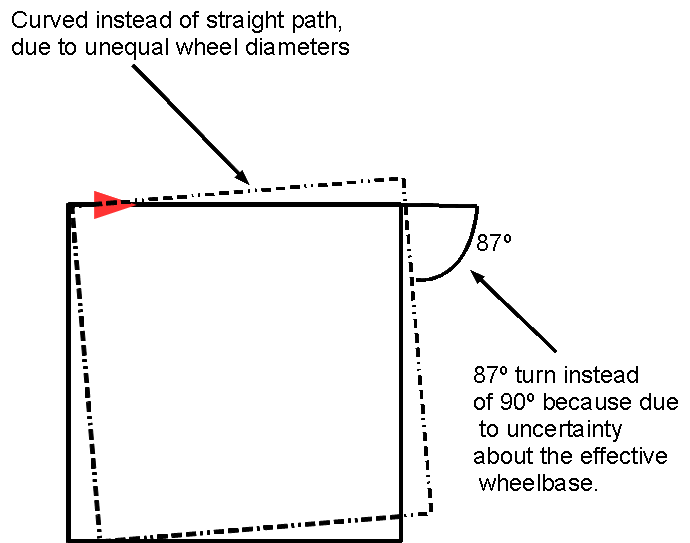
\includegraphics[width = 0.5\textwidth]{../../figures/sys_odometry_error} 
\caption{The effect of systematic odometry errors}
\label{sys_error}
\end{figure}

The paper by \textit{Borenstein et al.} describes the main danger about uncertainty of either the \textit{wheel diameters} or the \textit{wheelbase} as that modifying one of them can cause the other value to seem calibrated as well. This can be caused by using an \textit{unidirectional} square path as a benchmark test, which is what have been done in the beginning of this project, see \ref{mov_calibration} on page \pageref{mov_calibration} for more information. \\
The danger with this approach is that it is easy to analyse the odometry error being caused by either the wheel diameters, a slightly curved movement path, or the wheelbase which would caused over or under turning. \\
If only an unidirectional calibration approach is done either of these errors can be "fixed" by modifying either the wheel diameters or the wheelbase and the result would show a "correct" result.
For example if the actual movement path is as displayed by the dotted line in figure \ref{sys_error}, the movement error could be "fixed" by modifying the wheelbase which would led to robot turn, say 93$^{\circ}$, which would cause the path to appear correct. By doing that the path will look correct and thereby the robot calibrated, but in reality the robot overturns in order to compensate for the curved movement path.\\
However this will lead to increased odometry errors as the robot will appear to turn accurately but the odometry error is in reality caused by the uncertainty about the wheel diameters which leads to a curved movement path. Of course this can also happen the other way around.\\


\subsection{Bidirectional Square Path calibration: "UMBmark"}
As the preceding section shown an \textit{unidirectional} square path is unsuitable for testing odometry performance as it can easily conceal 2 mutually compensating odometry errors.\\
To overcome this problem, the paper introduces a \textit{bidirectional} square path experiment, called the \textit{University of Michigan Benchmark} or for short \textit{UMBmark}. 
In this experiment the robot moves both clockwise and counter clockwise in a square path. This way it easily shows the concealed odometry error which is caused when the robot has been calibrated by only an unidirectional approach.\\

\begin{figure}[h]
\centering
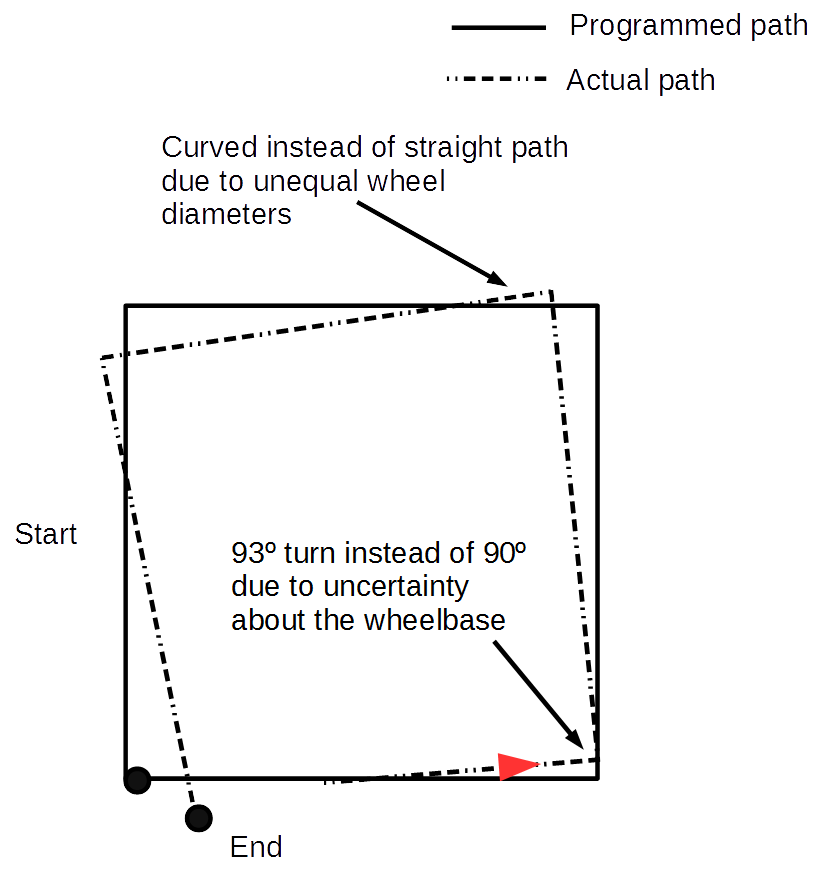
\includegraphics[width = 0.5\textwidth]{../../figures/unidirectional_error} 
\caption{The odometry error when the unidirectional path is performed in the opposite direction}
\label{unidirectional_error}
\end{figure}

Figure \ref{unidirectional_error} shows the result of running a robot which has been "calibrated" with the \textit{unidirectional} approach in the opposite direction. It shows clearly the short comings of such "calibration" as it now overturns in addition to the curved movement path.\\[3ex]

The paper describes methods which allow of accurate mathematical solutions to the given problems. But since the  Webots\textsuperscript{\texttrademark} simulator does not posses inbuilt tools to measure robot movement accurately no measurements can be taken to which would allow to follow this procedure.\\
What has been done to calibrate the E-Puck robot is to implement the UMBmark functions inside the project and run them, altering the \textit{wheel diameter} and \textit{wheelbase} values over time and compare the results.\\


\begin{lstlisting}[caption={The UMBmark experiment procedure}, label={UMBmark}]
double dSpeed = 300.0f; //movement speed
double dDistance = 0.5f;  //movement distance of 1 square. These distances have been changed over time

/**
University of Michigan Benchmark
*/
void UMBmark(double dSpeed, double dDistance){	
	//move the robot clockwise and counterclockwise 
	measure_clockWise(dSpeed, dDistance);
	
	measure_CounterClockWise(dSpeed, dDistance);
	
	stop_robot();
} 
/**
Function to measure the movement accuracy by driving
a clockwise square.
This is part of the UMBmark algorithm
*/
void measure_clockWise(double dSpeed, double dDistance){
	int i, j;
	
	for(i = 0;i < NUMTOURNAMENTS; i++){
		for(j = 0;j < 4;j++){
			move_forward(dSpeed, dDistance);
			turn_right(dSpeed);
		}
		wb_robot_step(TIME_STEP);
	}
}  

/**
Function to measure the movement accuracy by driving
a counter-clockwise square.
This is part of the UMBmark algorithm
*/
void measure_CounterClockWise(double dSpeed, double dDistance){
	int i, j; 
	
	//turn the robot right for moving the same square counter clock wise
	turn_right(dSpeed);
	
	for(i = 0;i < NUMTOURNAMENTS;i++){		
		for(j = 0;j < 4; j++){
			move_forward(dSpeed, dDistance);
			turn_left(dSpeed);
		}
		wb_robot_step(TIME_STEP);
	}
} 
\end{lstlisting}

Listing \ref{UMBmark} shows the code used for the UMBmark algorithm which is implemented inside the project. The start values are to move with a speed of \textit{300}, which is an acceptable speed as well as moving a distance of \textit{0.5}, which equals FIXME(check how many square this equals).\\
As a reminder the start values for the wheel diameters are:\\
$D_{R} = 0.0404 = 40.4mm$\\
$D_{L} = 0.0416 = 41.6mm$\\
Where $D_{R}$ represents the right wheel diameter and  $D_{L}$ the left wheel.\\
The value of the wheelbase is:\\
$0.052 = 52mm$\\ 

Firstly the amount of degrees which the robot turns when the \textit{turn\_left()} and \textit{turn\_right()} methods has been set from 100$^{\circ}$ to 90$^{\circ}$. The simulation was then been run 10 time times per test iteration to assure that the robot movements are not caused by random effects.\\
Between each iteration either of the wheel diameter and wheelbase values has either been decreased or increased in the simulation then been run for another 10 times. After each test iteration of 10 runs the value was either set back to its original value of the odometry error increased or if the error decreased the value was further changed. \\
At a later point when the odometry error seamed resolved multiple values were changed, in order to assure that they are correct. \\
The resulting result was that the wheel diameters are correct however the wheelbase value was updated from:\\
$0.052 = 52mm$\\ 
to:
$0.058 = 58mm$\\ 
As it is simple to check the current calibration for a curved movement error the robot was moved the whole length of the simulation range to confirm that the movement path is indeed straight and not curved, which it was. This was done to recheck that the result from the UMBmark calibration are correct. \\[3ex]

The paper suggest using larger movement patterns, where available, in order to check to correctness of the calibration. As this was easily done in the simulator the square was increased from 1x1 floor square to 2x2 and then 4x4. The results were largely the same, however by a square size from 4x4 the robot did not move full 4 squares. This shows that the squares on the floor, which until now have been expected to be FIXME(Check these values) 0.5 in code or equal to FIXME(add size), are not exactly that value but something close to it. \\
Because of the rest amount of time available was not big by the time of this calibration process the calibration results from 1x1 and 2x2 square paths have been deemed sufficient, rather than running multiple experiments trying to figure out the exact size of the squares. \\

\section{Reference point approach}
After the E-Puck values have been calibrated with the method described in the preceding section, the movement improvement has been checked in the development environment. \\

\begin{figure}[h]
\centering
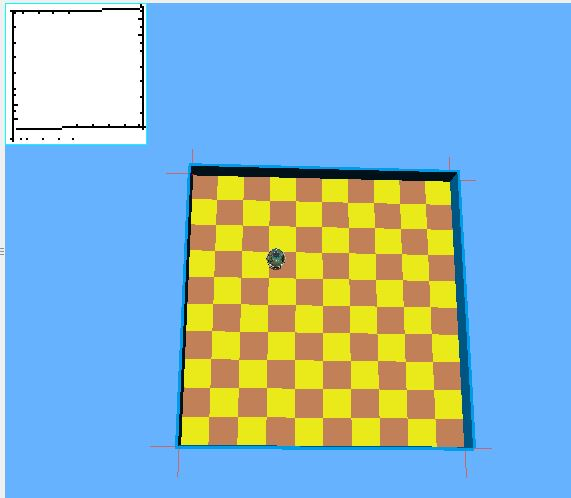
\includegraphics[width = 0.5\textwidth]{../../figures/odometry_error} 
\caption{Improved mapping with the calibrated robot, but the localisation error still persists}
\label{odometry_error}
\end{figure}

Figure \ref{odometry_error} shows the mapping result generated with the calibrated movement.\\
It shows that program is now able to generated a map of the environment with straight walls, compared to the much more skewed wall result which were generated before. 
FIXME(Rollback github repo and add screenshot about it)\\

However it is not entirely perfect at this stage as an localisation error still persists, as the robot while mapping the lower wall maps it inside the wrong place. \\
This is the result of noise generated inside the environment as well the nature of odometry calculations.
Odometry is always, in best case, an estimate of the localisation, this combined with noise and friction inside the simulator environment caused the robot to never turn 100\% accurate. \\
The algorithms implemented until this point, which compare the heading of the robot and turn it to fit the wanted heading as well as the recalibrated movement algorithms made huge improvements to the robots movements.\\
But still a minimal odometry error persists, which accumulates over time and cause the odometry error which can be seen in figure \ref{odometry_error}. \\[3ex]

At this point the use of reference points was considered in order the fix the localisation problem.\\
The approach taken for the reference point was to use the corners of the room as reference points.
This would be achieved by creating new functions and a \textit{struct }which use the already existing corner localisation implemented inside the U-Turn routine and save the X and Y coordinates the robot has calculated. 
That way the robot can reset it's X and Y coordinates to the coordinates previous saved inside the struct once the same reference point is reached again.\\












 





\chapter{Testing}
\label{Testing}
This chapter holds the overall testing results and test information about the final program.
During implementation the program was only ever run in a single environment, \textbf{room 1}.
In this chapter the results of running the program in different environments are documented. The environments differ in shape and size as well as well as in obstacle population.

\section{Overall Approach to Testing}
As the program requires an simulator to be run in, it is not possible to test the program in any other way than to run it in an simulator and document the results. This factor makes also automatic unit testing impossible. During implementation the program was only ever tested in a single environment called \textbf{room 1}. All changes which were done to the code and problems which were documented in early chapters have been the result of the robots performance in this environment. \\[3ex]

The reason the program was never tested in different environment during implementation was since the program was not complete enough, it was assumed that before the program can be tested in multiple environments a solution for a simple environment must exist.\\
It is worth noting at this point that the project is considered finished as the mapping results for the environment it was developed for are satisfactory. However the program could still be improved in future implementations, which is also needed as the program does not perform in different environments as well as it could do if more time for further implementation would have been available. 
This is discussed further in the following sections.

\section{Test environment: Room 1}
\label{room1}
Room 1 is the "original" environment in which the program was implemented. \\
It is a simple, empty, room which size is 10x10 squares, figure \ref{room1_empty} shows this environment. In order to measure the environment size the chess board pattern which makes up the floor of the simulator environment is used to measure it. Each \textit{square} measures 10cm x 10cm.

\begin{figure}[h]
\centering
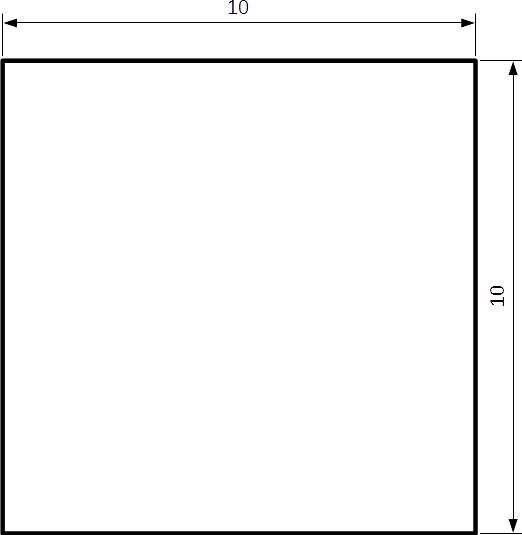
\includegraphics[width = 0.5\textwidth]{../../figures/room1_empty.png}
\caption{Room 1 empty test environment}
\label{room1_empty}
\end{figure}

\subsection{Obstacle free test}

The results gathered in this test environment, as it is the simplest, as well as the environment in which the program was developed are by far the best in from of final result. \\

\begin{figure}[h]
\centering
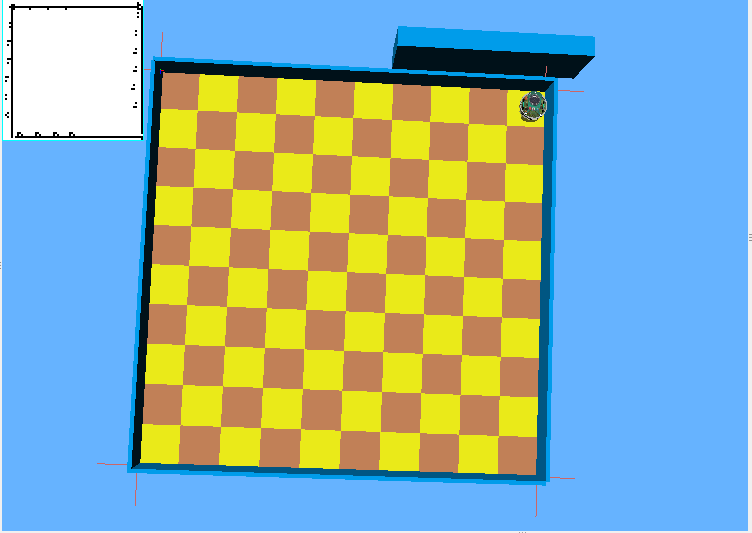
\includegraphics[width = 0.5\textwidth]{../../figures/map_results/result_room1_empty.png}
\caption{Room 1 empty environment result}
\label{room1_empty_result}
\end{figure}

Figure \ref{room1_empty_result} shows the result of the environment after the map has been "closet". The resulting map clearly depictures the spotty nature of the U-turn mapping which is described in Chapter 3 subsection \ref{deployment_improvement} on page \pageref{deployment_improvement} . \\[3ex]

The generated map shows that the program is able to generate straight and accurate mappings of an environment as long as the robot is able to reset its odometry values at some point during the run. More info of what can happen if the odometry is not reset can be found in chapter 3 section \ref{ref_point_approach} on page \pageref{ref_point_approach}.\\
The reason of why the program performs this well in the test environment compared to other environment is that is able to reset its odometry values by passing \textbf{corner 1}, before it moves to the uncharted \textbf{corner 2}. More information about the corner approach can be found in chapter 3 section \ref{ref_point_approach} on page \pageref{ref_point_approach}. \\
That the accumulated odometry error was growing constantly during program runs can be seen at the placement of the spots of the u-turn routine, these spots are marked red in figure \ref{room1_empty_marked}.

\begin{figure}[h]
\centering
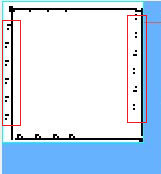
\includegraphics[width = 0.5\textwidth]{../../figures/room1_result_marked.png}
\caption{Room 1 map result with marked odometry dislocation}
\label{room1_empty_marked}
\end{figure}

If these spots are compared to the one at bottom and top site of the generated map, it can be clearly seen that the odometry location error was crowing, and became very noticeable after the map had been generated about 50\%.\\[3ex]

However the odometry location error was reset as the robot reached \textbf{corner 1}, which X and Y coordinates were saved as the robot traversed said corner for the first time. \\
This reset the odometry values of the odometry struct and made it possible to continuously map the environment with good results. \\
Figure \ref{odometry_error} on page \pageref{odometry_error} shows the localisation error if the odometry values are not reset.\\[3ex]

However this test environment is not without shortcomings either. If the program is allowed to keep working and mapping the environment the odometry error is increasing again.\\

\begin{figure}[h]
\centering
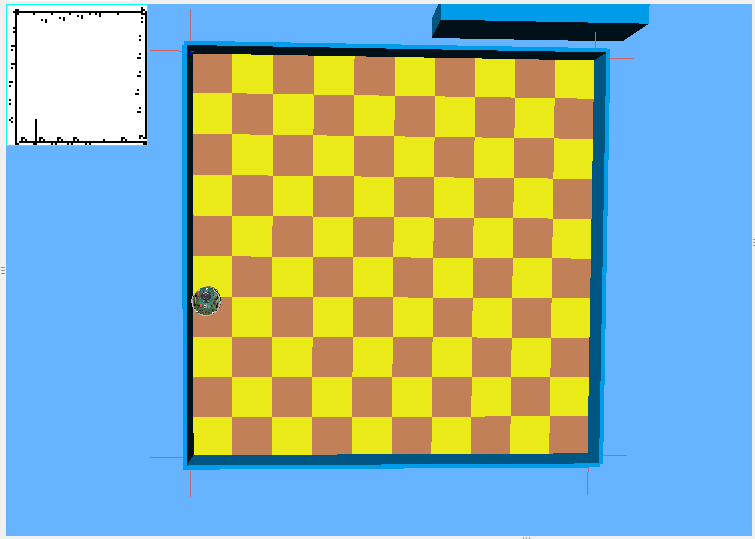
\includegraphics[width = 0.5\textwidth]{../../figures/map_results/odometry_error_and_reset.png}
\caption{Room 1 map result with crowing odometry error}
\label{room1_empty_reset}
\end{figure}

Figure \ref{room1_empty_reset} shows the accumulated odometry error after the environment has been traversed approximately 2 times. \\
As can be seen in this figure the odometry location error keeps accumulating even though it has been reset a few times, at \textbf{corner 1} and \textbf{corner 4}. But the mapped line which can be seen on the lower left corner of the generated map indicates that the localisation error became to big so  that an area was map in the middle of the environment which clearly belongs to the left hand wall.
This however is also an working example of the reset function which has been implemented for the corners of the environment. As the location information of the odometry struct have been reset as the corner was reached. The reset can be seen as the robot depicted in the figure already did another pass along the left hand wall up and down, after being reset in the lower left corner. \\[3ex]

This localisation error however is a rather random event, as different results from other runs suggest that the odometry error is strongly based on the random nature of the noise in the simulator.

\begin{figure}[h]
\centering
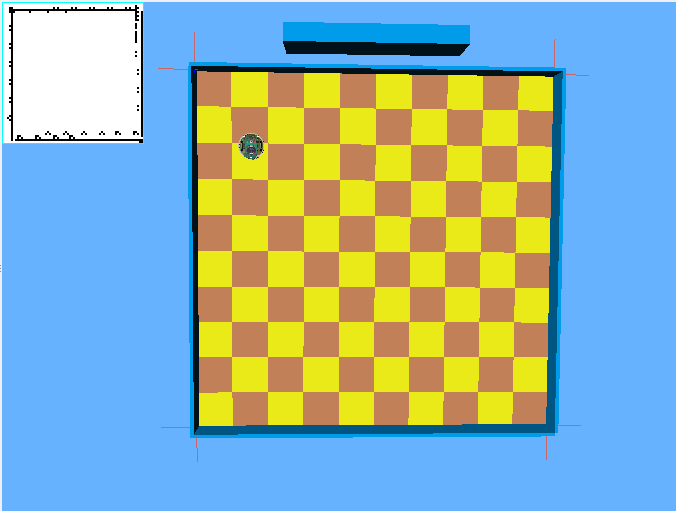
\includegraphics[width = 0.5\textwidth]{../../figures/map_results/simulator_noise_mapping.png}
\caption{Room 1 map result with different odometry error}
\label{room1_simulator_noise}
\end{figure}

Figure \ref{room1_simulator_noise} shows the result of another test run, here the robot only had a small miss mapping issue in the upper-right corner of the map, which happened right after the map was closed. However this error was only in a small area, and was completely reset when it reached the lower-right corner of the environment. The test run depicted in this figure has progressed further than the test run shown in figure \ref{room1_empty_reset}, and it shows that the odometry localisation error did not happen again, in the same place.\\
In other test runs the odometry localisation error did not happen until the robot started traversing the environment the 3rd time, however 90\% of times before it happened during the 2nd environment traverse, this suggest that the problem lies within the random nature of the simulator, however that this random nature is within boundaries.

\subsubsection{Conclusion for this test environment}
While the mapping performs reasonably well within this test environment not all test runs are the same. The mappings differ minimal in places every simulation run, this happens because of the random nature of the simulator. \\
While the mapping of the whole environment can be performed with reasonably similar results, the results start to differ a lot more when the robot traverses the environment a 2nd or 3rd time. The figures \ref{room1_empty_reset} and \ref{room1_simulator_noise} are the results of 2 different simulator runs which happened directly after another. Other times the 2nd simulator run returned no mapping error which was more noticeable than the common minor dis-localisation, but major errors as shown in these figures happened in later runs. The mapping error de-pictured in both documents that while the simulator random nature causes minimal map differenced every time, larger errors happen more seldom and more randomly.

\subsection{Environment with obstacles}
\label{room1_obstacles}
This subsection shows and describes the results of another test environment. \\
This environment is the same as described in the previous sub-section however this has an obstacles added to it.

\begin{figure}[h]
\centering
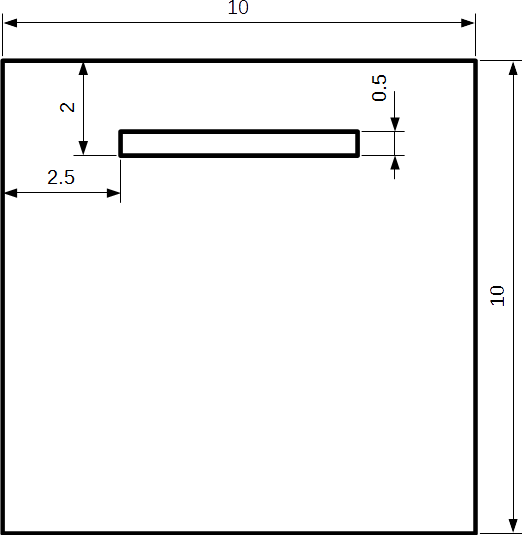
\includegraphics[width = 0.5\textwidth]{../../figures/room1_obstacle.png}
\caption{Measurements of room 1 with obstacle added to it}
\label{room1_obstacle}
\end{figure}

Figure \ref{room1_obstacle} shows the measurements and location of the obstacles added to the environment, again all measurements are in \textit{squares}.

\begin{figure}[h]
\centering
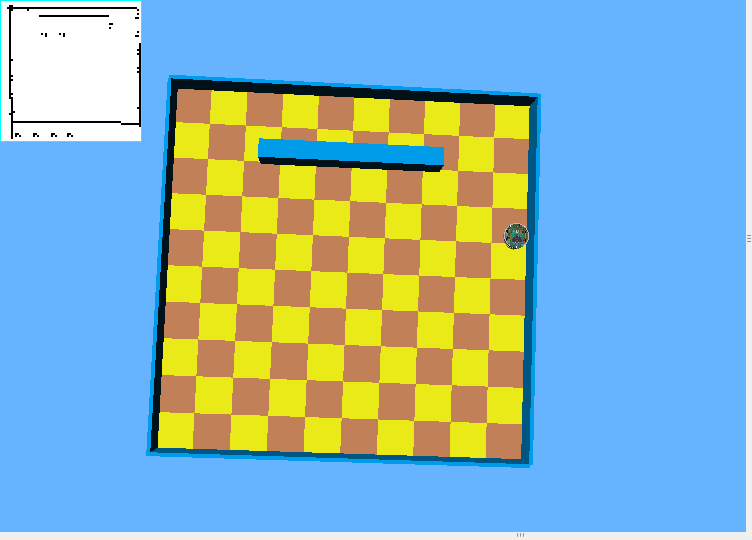
\includegraphics[width = 0.5\textwidth]{../../figures/map_results/one_obstacle_save_error.png}
\caption{Room 1 with obstacle map result}
\label{room1_obstacle_result}
\end{figure}

Figure \ref{room1_obstacle_result} shows the result for this environment.\\
As it can clearly be seen, this figure shows the major shortcomings of the final program. On the lower part of the generated map, it can clearly be seen where the major shortcoming of this solution, the odometry localisation error gets too big. \\
Unlike to the \textbf{room 1} example without any obstacle, which is described in the previous section, this result depicts what happens when the robot is not able to reach a saved reference point(already traversed and saved corners), but rather continues mapping without being reset. \\[3ex]

What has happened in this case is that the obstacle prevented the robot to traverse the whole width of the map, which altered the movement enough for the robot to reach the unsaved lower-right corner of the map before it reached an already saved reference point which would led to the localisation information being reset. \\
This can cause a couple of problems. The biggest of them is, which can be clearly seen, that the localisation error gets too large for the map to be usable. The problem in this case is that the odometry information of the lower-right corner are saved, and every time the robot passes this corner the odometry information will be updated to the saved, wrong, information.\\[3ex]

Besides this major error, it also shows the programs shortcomings in the mapping of obstacles which are placed in the middle of the room. 

\begin{figure}[h]
\centering
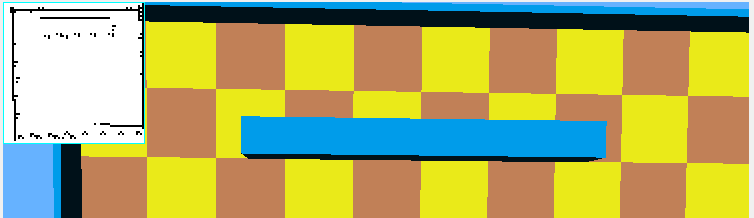
\includegraphics[width = 0.5\textwidth]{../../figures/map_results/obstacle_mapping_error.png}
\caption{Obstacle mapping shortcomings}
\label{obstacle_mapping_error}
\end{figure}

Figure \ref{obstacle_mapping_error} shows the problem when an obstacle in the middle of the room is being mapped with the current mapping approach. \\
The upper-side of the obstacle is mapped reasonable well, however the the other sides are lacking. There are some spots on the right side of the obstacle which have been marked by during the U-Turn routine, however the lower-side of the obstacle shows the real shortcomings. When the mapping of the lower and the upper side of the obstacle are compared it gets clear that the main limitation with this approach is the usable mapping only happens when the robot traverse the obstacle which its side to it, so that it will be mapped. The spotty mapping points generated by the U-Turn routine are usable to outline the obstacle at best, however the specific movement pattern implemented in this project can prevent possible mapping of an obstacle should the obstacle be placed at a point which will not be passed by during the robot movements pattern. \\[3ex]

Another problem is the odometry error in an environment like this. As has already be shown the localisation error gets to big and the altered movement pattern prevents the robot from resetting its localisation values, that is not without it getting reset to something wrong when it passes a long the reference point which has been saved with the wrong odometry data in the first place, in this case the lower-right corner. \\
This however does not only cause errors for the outline of the environment but also for the obstacles, as in some simulation runs visible localisation difference on the spotty outline of an obstacle can be seen. \\[3ex]

\begin{figure}[h]
\centering
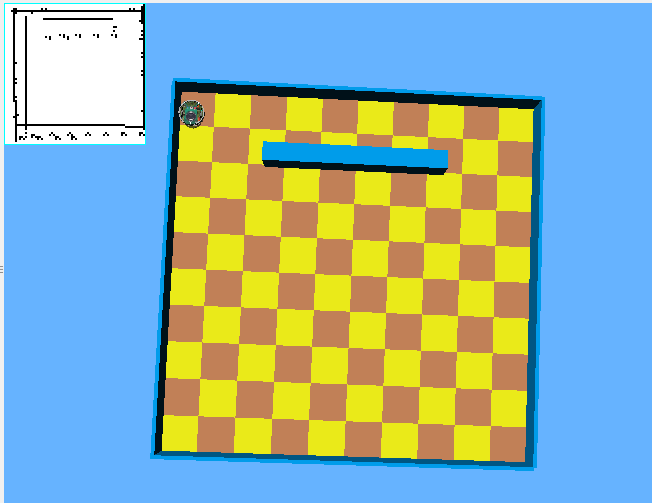
\includegraphics[width = 0.5\textwidth]{../../figures/map_results/one_obstacle_odometry_error.png}
\caption{Accumulated odometry error}
\label{one_obstacle_odometry_error}
\end{figure}

Figure \ref{one_obstacle_odometry_error} shows the map result at a later point during the environment traverse. The figure shows how much the localisation errors accumulate  over time when the robot is not able to reset its localisation values. \\
It shows the already discussed localisation error for the lower side of the map, as well as the spotty outlining in the obstacle. However this map shows also that the localisation values have been reset in the corners which were passed before the localisation error became to big, as the spotty mappings on the lower side of the map show. While the entire lower wall of the environment is mapped at a wrong place, the localisation values have been reset in the upper right corner which causes the spotted, U-Turn based,  mappings along the lower right hand side.\\

\begin{figure}[h]
\centering
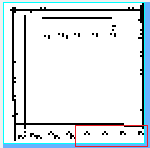
\includegraphics[width = 0.5\textwidth]{../../figures/map_results/dotted_odometry_error.png}
\caption{Marked spots}
\label{dotted_odomery_error}
\end{figure}

In figure \ref{dotted_odomery_error} these spots have been marked. The spots to the left hand side of the marked spots have been mapped after the robot had started, since it starts in the center of the map facing to the lower end of the environment. \\
As the marked spots are approximately at the Y axes as the other markings, can be seen that the robot resets its localisation values to the correct values when it passes the upper-corner reference point. \\
However this figure also depicts what the accumulated odometry errors cause to an already scanned side. On the left hand side of the figure it can easily be seen where the robot remapped the left hand wall of the environment.\\

\subsubsection{Conclusion for this test environment}
This test environment shows the shortcomings of this program, the static movement pattern can cause problems when mapping obstacles as the robot will only ever move in the same movement pattern. This however can, and in most cases will, lead to an large accumulation of localisation error.\\
It is apparent that the major problem of this program is that the odometry values need to be reset in given intervals in order to prevent an to large accumulation of errors. This is however, with the current solution, only possible when the robot manages to pass by an saved reference point before the localisation error either becomes to large, or another reference point is set with the wrong localisation information.\\[3ex]

There are a couple of ways the problems which become apparent in this test environment could have been fixed. One possibility is to have a wall following algorithm which allows for the mapping of the outline of an obstacle before falling back into another movement pattern. \\
This would prevent problem with the mapping of obstacle which has been discussed in the previous section. Another solution would be to set reference points more often, or have a way of localizing the robot besides having set reference points, possibilities for this would be GPS or long range scanners which are able to keep track of global reference points, which have been set previous to the run.\\
There are a couple of possibilities which could have been implemented in order to make this mapping better, however the problems encountered during implementation have taken to much time to fix to be even able to map a single, empty, environment to be able to implement further algorithms after test runs had been done for environment with obstacles inside them.

\section{Room 2}
Room 2 is an narrower version of \textbf{room 1}, with a size of 6x10 squares.

\begin{figure}[h]
\centering
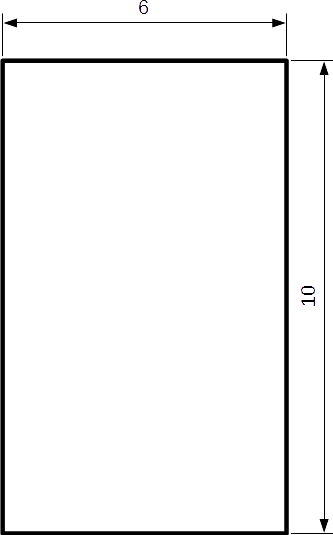
\includegraphics[width = 0.5\textwidth]{../../figures/room2_empty.png}
\caption{Room 2 measurements}
\label{room2_empty}
\end{figure}

\subsection{Obstacle free test}
In this section the results for the obstacle free version of \textbf{room 2} will be shown and discussed. \\[3ex]

\begin{figure}[h]
\centering
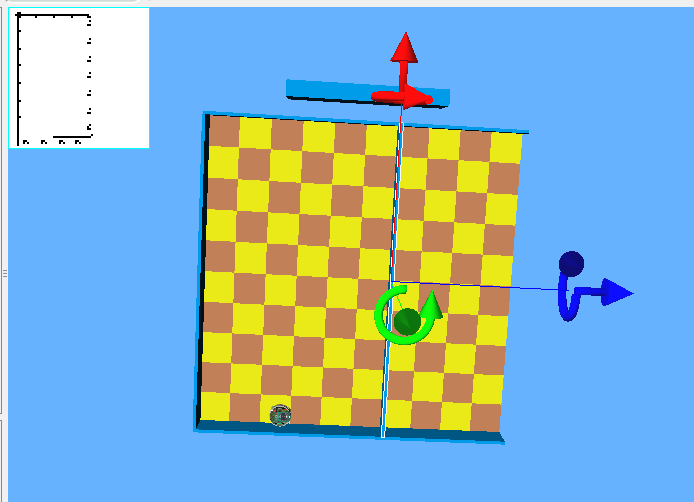
\includegraphics[width = 0.5\textwidth]{../../figures/map_results/save_corner_with_odometry_error.png}
\caption{Room 2 results}
\label{room2_results}
\end{figure}

Figure \ref{room2_results} shows the result of the second test environment.
While the map is not finished, the robot was stuck in an eternal loop at the lower wall of the environment.\\
This environment shows once more that the mapping works fine as long as the localisation error has not accumulated it self to much. \\

\begin{figure}[h]
\centering
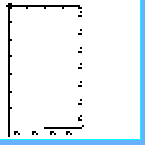
\includegraphics[width = 0.5\textwidth]{../../figures/map_results/minimum_localisation_error.png}
\caption{Room 2 shows that the localisation error depends on environment size}
\label{room2_error}
\end{figure}

However figure \ref{room2_error} documents also that the increase of the localisation error strongly depends on the size of the environment and there by how far the robot traverses between each wall. \\
The localisation error strongly changes when the robot driver longer distances, even on straight lines. Even if the robot is perfectly calibrated which prevents curves movement caused by different wheel diameters (more on this can be found in chapter 3 section \ref{recalibration} on page \pageref{recalibration}), the robot will never turn an exact amount of degrees, this is caused by the friction between the wheels and the floor. \\
This however, as already discussed in chapter 3, leads to the robot believing it is somewhere while it actually is somewhere else.  As figure \ref{room2_error} documents this error is reduced if the robot does not need to drive far until it has to turn again.\\
It does so by showing clearly that localisation error, while it still persists, is much smaller than in an empty environment where to robot has to drive further distances until turning. An example of this can be seen in chapter 3 section \ref{ref_point_approach} on page \pageref{ref_point_approach}. \\[3ex]

\begin{figure}[h]
\centering
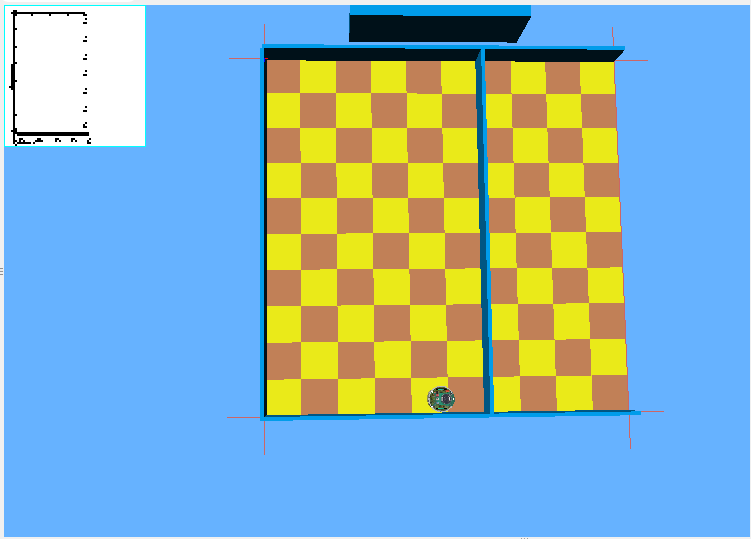
\includegraphics[width = 0.5\textwidth]{../../figures/map_results/save_corner_with_odometry_error_later.png}
\caption{Room 2 results at a later point}
\label{room2_results_later}
\end{figure}

However the localisation error is not the only problem. As can be seen in figure \ref{room2_error} also in this case the robot reaches an uncharted reference point before passing by an existing reference point to reset its localisation values. This leads to the same problem encountered in section \ref{room1_obstacles}. \\
However the robot in this case is stuck within an eternal loop, where it resets to the right coordinates at the lower-left hand corner and drives to the right-hand side of the map where it gets reset to the wrong localisation values again. \\
The problem of this happening is a bug inside the code combined with odometry errors. The odometry error causes the robot to not directly drive close to the wall but rather stay a bit away from it. And the bug causes the robot to not change it overall direction whenever it reaches one of the corners but rather to stay in the U-Turn movement pattern.

\subsubsection{Conclusion of this test environment}
This test environment did not really showcase any other problems with code then the ones already covered in section \ref{room1}. It did however show case an until now unknown bug which would need to be patched out, if more time were available.\\
This test environment however documented, the already existing assumption, that the size of the localisation error depends on how long distances the robot needs to move until turning again. This localisation error in the first place is however caused by inaccurate turning caused by friction in the environment.

\subsection{Environment with obstacles}
In this subsection the test results an environment which has the same size as \textbf{room 2}, however holds an extra obstacle.\\

\begin{figure}[h]
\centering
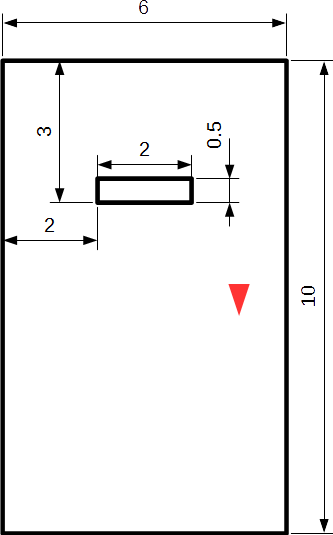
\includegraphics[width = 0.5\textwidth]{../../figures/room2_obstacle.png}
\caption{Room 2 with obstacles measurements}
\label{room2_obstacles}
\end{figure}

Figure \ref{room2_obstacles_result} shows the result of this test environment. \\
As it can clearly be seen the map of this environment is not finished, the reason for that are bugs in the code and odometry errors.
The robot starts at the marked starting position, red arrow, and proceeds to map the environment as usual. It can clearly be seen where the robot mapped the outline of the obstacle as it passed it. When the robot passed the upper-left reference point this point is saved as usual. \\
The robot then maps the left-hand side wall of the environment, and saves the lower-left hand corner as usual.\\

\begin{figure}[h]
\centering
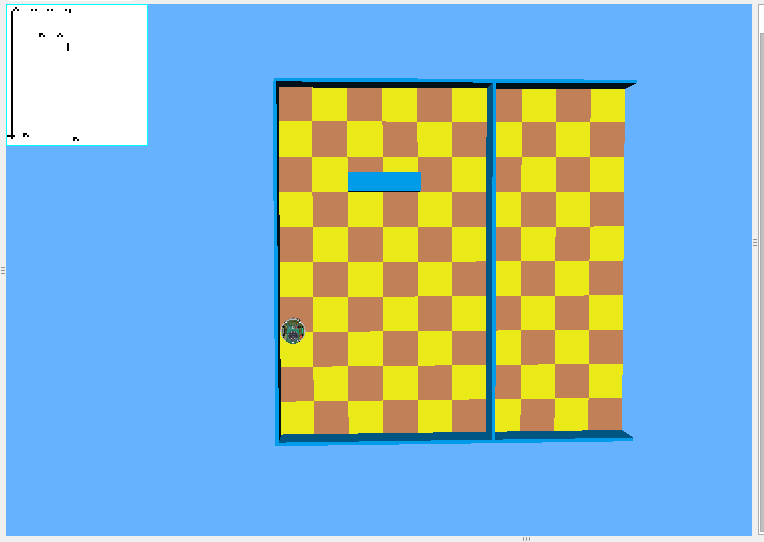
\includegraphics[width = 0.5\textwidth]{../../figures/map_results/room_2_obstacle_result.png}
\caption{Room 2 with obstacles result}
\label{room2_obstacles_result}
\end{figure}

However here is where the bug in the program causes the robot also save the same corner as the lower-right hand corner and change the direction value of the odometry struct to west wards, while the robot is actually moving north warts.  \\
Figure \ref{room2_saving_error} shows the readout generated by the program. It shows how the robot,correctly, moved southwards then saved the corner as corner 1, which is also correct, but then saves the corner also as corner 2 and sets its own direction to west ward, while actually moving to the north.\\[3ex]

This robot then proceeds to move upwards along the left-hand side wall, however the mapping the robot does is outside the map area as it believes to move west ward. The robot drives ~1/4 of the the environment size upwards before the simulator crashes. This crash has happened every single time this environment was tested.

\begin{figure}[h]
\centering
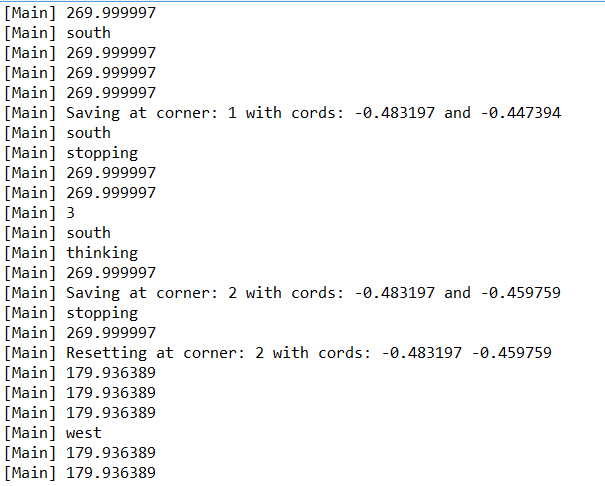
\includegraphics[width = 0.5\textwidth]{../../figures/map_results/room2_saving_error.png}
\caption{Buggy software causes causes the robot to save wrong values}
\label{room2_saving_error}
\end{figure}

\subsubsection{Conclusion of this test environment}
This test clearly showcases another major bug within the program. Unfortunately not more information can be gather from the test runs as the simulator crashes every time at the same place.

\section{Room 3}
This section holds the description and results of test of environment \textbf{room 3}. \\
This test environment differs from the previous test environments as it is a more "complex" environment compared to the others. It is more complex as it is completely square, this is done to test the programs performance in a environment like this.\\
This section was also not tested with obstacles inside it. The reason being that the previously gathered data shows that obstacle inside the room disturb the mapping and prevent a complete mapping.
Figure \ref{room3_empty} shows the environment and its measurements. \\

\begin{figure}[h]
\centering
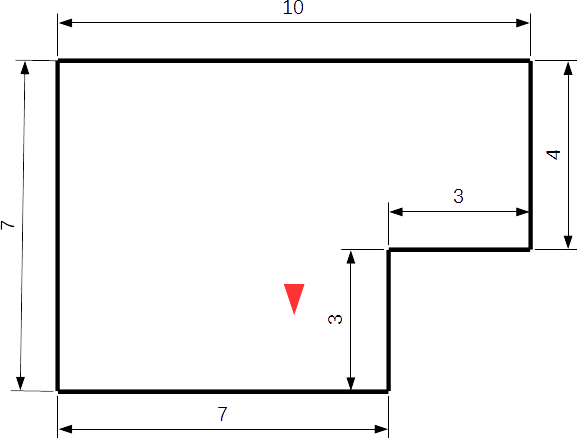
\includegraphics[width = 0.5\textwidth]{../../figures/room3_empty}
\caption{Measurements of room 3}
\label{room3_empty}
\end{figure}

Figure \ref{room3_result1} shows the map result after the robot traversed a part of the map. It can be seen that the robot mapped the outline of the right-hand wall, however it can be clearly seen that the localisation error accumulated to much which prevents an accurate mapping of the lower wall. \\

\begin{figure}[h]
\centering
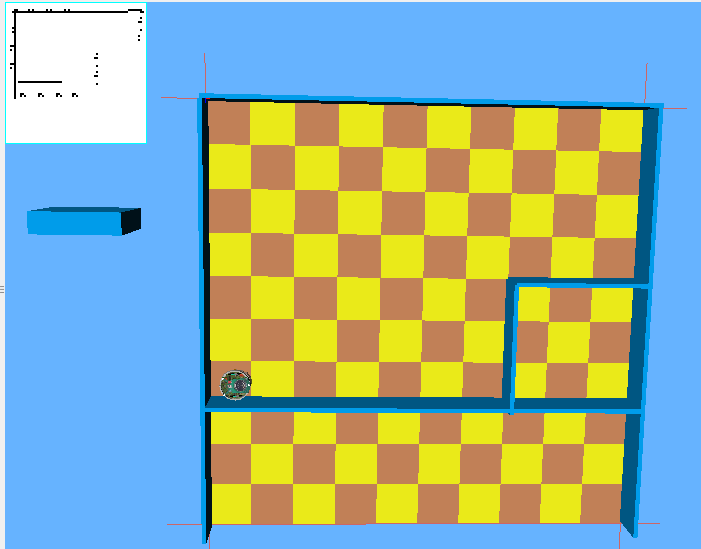
\includegraphics[width = 0.5\textwidth]{../../figures/map_results/room4_result1.png}
\caption{Result of the third room}
\label{room3_result1}
\end{figure}

It resets the localisation values at the lower left corner, however then proceeds to reset the values to the equivalent of the upper-right corner immediately. The robot then starts to move back and forth along the lower wall, then proceeded to move up the left wall. \\
It resets the localisation values again when the lower-left hand corner is reached for the second time, then moves upwards along the left wall, however the odometry struct now holds the wrong orientation values: the robot believes to move east(to the right).
The robot then proceeded moving along the walls in the normal movement pattern, however with the localisation and orientation values all wrong the mapping was unusable, and the test was ended at this point.

\subsection{Conclusion of this test environment}
This test environment did not produce a lot of new insight into the final program. While it documented the shortcomings of the reference point algorithm this is not new data, as previous test environments showed the same data. \\
The partly created map with can be seen in figure \ref{room3_result1} indicated that the mapping process of the wall formation at the lower right side of the environment would have been lacking at best. This is based on the moving pattern where the robot moves given distances in the turns, should an wall or obstacle not be "luckily" lay to the side of this path chances are that the robot will not be able to map it, in best cast map the outline. \\

\section{Conclusion}
The test results inside this chapter give clear insight into the weak and strong sides of the program.\\
Unfortunately there are more weak points. During the implementation phase of the project a couple of problems were encountered, problems with odometry, localisation and mapping. While these problems were countered and fixed the solution seamed good inside the implementation environment. This is the main reason why some of the programs shortcomings exist.\\[3ex]

The algorithm which handles the reference points is based on prior knowledge which was gathered during test runs in the implementation phase. It was known prior to design of the algorithm in which direction the robot is moving and from what direction it will approach a corner of the environment. This approach works fine inside the \textbf{room 1} environment but \textbf{room 2} and \textbf{room 3} have shown that this approach failed if the robot should move in a slightly different path than to the one the algorithm was designed under. \\
If the robot reaches a corner but its direction is different from the one specified in the algorithm, it will set or reset its localisation values to different corners than it should. This problem however could be fixed by adding more control statements to the algorithm, rather than simple approach which is implemented at this moment. \\[3ex]

Another weak point of the program is the movement pattern, if obstacles are placed inside the environment their presence can disturb the movement pattern enough to cause severe odometry and localisation errors. It has been observed in the testing phase that an E-Puck has collided with the wall, but rather than to stop it continued driving, however skewed itself along the side of the obstacle changing it path and increasing the localisation error. While this can happen because of the absence of bumper sensors of the E-Puck robot platform and the placement of the distance sensors around the E-Puck's top side, it shows that this robot platform is not the best suited for map building.\\
Another example is the mapping of\textbf{room 3 }which can be seen in figure \ref{room3_result1} and the obstacle mapping of \textbf{room 1} from figure \ref{obstacle_mapping_error}. These 2 figures show the problems with the current movement pattern on walls and obstacles. There is no direct way of fixing the movement pattern in this program. One approach could be to add a wall-following algorithm to whenever a new obstacle is detected, or in case a completely different approach, some of them were discussed in Chapter 1 and 2. \\[3ex]

The biggest problem however is the localisation approach. \\
The localisation error accumulated over time and needs to be reset at some points during the program run in order to prevent large mapping errors which can be seen in all test cases. One of the aims with this project was to be able to localise the robot without the need of GPS or Compass data or long range scanners which can keep track of global reference points at all times. However odometry calculations , which is what was used to locate the robot in this project, have limitations. In a non-perfect environment(an environment without friction or sensor noise) odometry calculations are always going to be an estimate at best, this was the biggest challenge of this project from the very beginning. Without functioning odometry algorithms it was not able to turn the robot an accurate amount of degrees or move it a given distance, even though these algorithms were successfully implemented they are not 100\% accurate, because of friction and sensor noise. \\[3ex]

Without the ability to calculate how much the robot has moved or turned it was impossible to locate the robot accurately.
The localisation and movement algorithms in them self function perfectly, however since odometry calculations are really just estimated odometry and localisation errors accumulated over time. Functions were created to tackle these problems, algorithms which check the robots heading and ensure it is only ever deviating with a maximum threshold from their path, and to set reference points at points the robot is able to locate, the corners. However the algorithm which controls the heading is only ever accurate as long as the calculated orientation values are right, extreme odometry errors or collisions with walls/obstacles can lead to errors, as the robot posses no possibility to check the actual position and heading in the simulator\footnote{While it is possible to include API functions which return accurate localisation and rotation informations on the virtual robot such functions were never used as they would break the challenges and key points of this project.}.\\
Even considering a case where the heading control algorithms work completely fine(in most cases they do) the localisation error still increases over time. The algorithm designed to set reference points and reset the robots localisation values helped with this problem, however the short comings of this algorithm has already been discussed. \\[3ex]

The overall conclusion drawn on the localisation problem is that is possible to calculate a robot positions, to an extend. However the error will always become to big, and reference points set by the robot it self are unreliable.  While it is completely possible to use odometry calculations to tackle the localisation problem it is necessary to use predefined reference points or GPS and compass data. In order to use predefined reference points very strong and accurate sensors are required, which are not found for each robot platform, as well as the structure of the environment. GPS and compass data would make the localisation as accurate as possible. Of course GPS sensors have also a limited accuracy but the result will certainly be better than without GPS data. An possible approach could also be to combine GPS and odometry calculations to decrease the localisation error as much as possible. \\[3ex]

To summarize the overall conclusion of this project it can be said that, while the program does not perform well or manage to generated accurate maps(unless it is \textbf{room 1}, it has certainly been a learning experience. It has shown the limitations of solely odometry based systems and have given some insight in how to minimize odometry errors, even though it is impossible to remove them completely. \\
The program in itself has strong problems, the movement pattern is far from optimal, but ideas and insight on this was gathered as well. The test have shown the limitations of the implemented algorithms as soon as it was tested on more complex environment, but also provided informations on these shortcomings and ideas on these could be fixed in the future.

\chapter{Future Plans}
\section{Communication}
While it is possible to transfer information easily between robots since a simulator is used one keypoint was to try implement it as close to a realistic scenario as possible, meaning that the communication range for the robots is limited. In an realistic scenario every robot would have to send the acquired map back to the static start point/lead robot so that an overall map of the environment can be created. \\
Since the communication range for such small robots is limited and can be even further obstructed through obstacles like walls it is important to designated some robots as communication nodes. Such comm nodes would than remain stationary and link the "scout" robots, which do the exploration, back to do the lead robot. \\
Obviously the most effective way to do this is by implementing different behaviour patterns for scouts or comm robots, and implement a decision model which allows the robot to change between either pattern as the needs of the swarm change. E.g. in the start of the exploration no comm robots will be needed as the robots would most likely be inside the comm range of the lead robot, though this may change if the swarm is big and spread out enough. \\[3ex]

To surpass the problems of obstacles obstructing the communication the comm robots would need to position them self on logical places i.e. in order to scan a room it would be important that a comm robot places it self inside, or close to, the doorway so that others can explore the room and still communicated back to the rest of the swarm. The robot would need to stay inside the doorway as signals can not always travel through walls and the energy reserves of mobile robots are limited so they most likely can not send high power signals. \\
It has not been decided how this would be implemented since as of now it is not sure if the E-puck models implemented inside the simulator are able to send signals to other robots. While it is possible  to transfer signals through the E-puck's laser sensors it is not know if this would actually be a better implementation than using radio transmitters and receivers.\\[3ex]

The theory of what could be  implemented uses a defined maximum communication range for the robots and a grouping strategy which specifies that each scout robot need to stay in contact which at least 1 comm robot while the comm robots always need at least 1 other comm robot inside their communication range. If implemented correctly the comm robots would on this way create a communication link back to the lead robot/starting location which the scout robots can use to transfer all new information back.\\

\begin{figure}[h]
\centering
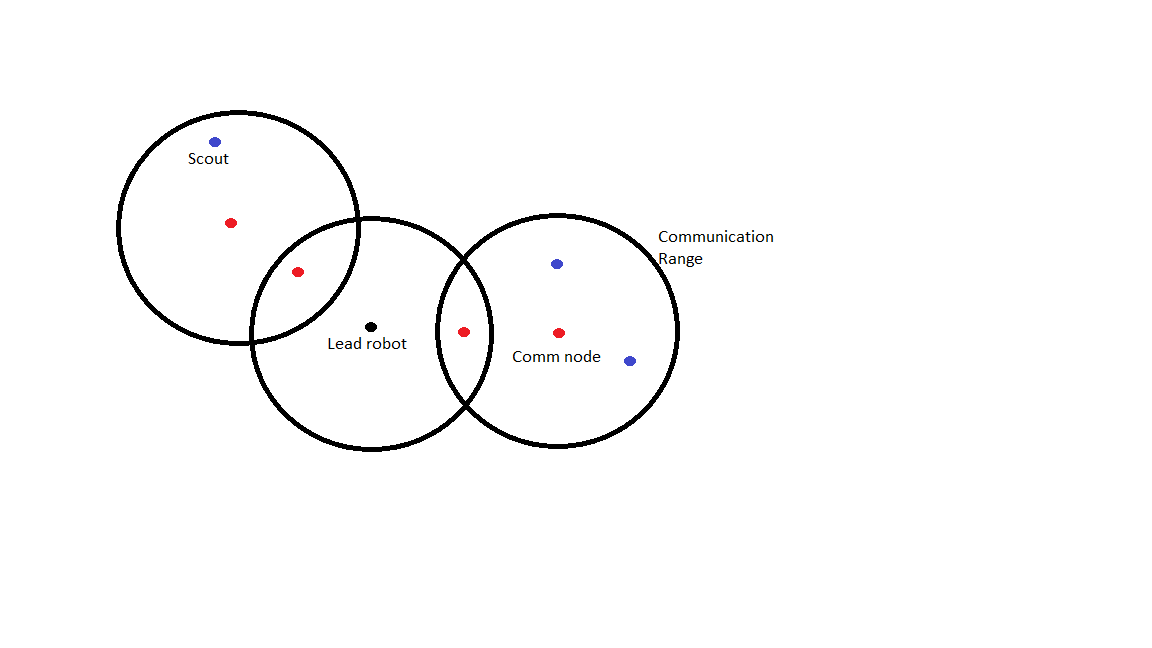
\includegraphics[width = 0.8\textwidth]{../../figures/comm_example.png} 
\caption{An example of the communication link}
\label{Figure 1}
\end{figure}

Figure 1 shows one possible example of the communication link, where the lead robot/ or in some cases a stationary uplink point is in the center and the communication robots(in red) placed in such positions that their comm range overlaps the comm range of other robots and the lead robot. \\
This configuration allows the scouts(in blue) to move and explore anything inside the communication range of the different comm robots. When the robots at the right side of the figure would now try to move outside the comm range one of them would have to change their behaviour pattern to "communication mode" at the outer range of the other comm nodes range while the last remaining scout continuous exploring in this direction. \\
This example shows that it is important to have a swarm of a suitable size for an environment to be able to cover at much area with the robots at hand and for cases in which this is not possible to be able to move the whole swarm in one unified direction to explore unmapped locations. This is however only doable when there is a lead robot since a stationary comm/uplink point is by definition, stationary.\\
\chapter{Evaluation}

Examiners expect to find in your dissertation a section addressing such questions as:

\begin{itemize}
   \item Were the requirements correctly identified? 
   \item Were the design decisions correct?
   \item Could a more suitable set of tools have been chosen?
   \item How well did the software meet the needs of those who were expecting to use it?
   \item How well were any other project aims achieved?
   \item If you were starting again, what would you do differently?
\end{itemize}

Such material is regarded as an important part of the dissertation; it should demonstrate that you are capable not only of carrying out a piece of work but also of thinking critically about how you did it and how you might have done it better. This is seen as an important part of an honours degree. 

There will be good things and room for improvement with any project. As you write this section, identify and discuss the parts of the work that went well and also consider ways in which the work could be improved. 

Review the discussion on the Evaluation section from the lectures. A recording is available on Blackboard. 

% add any additional chapters here

\setemptyheader
\addcontentsline{toc}{chapter}{Appendices}
\chapter*{Appendices}
\pagebreak

% start the appendix - sets up different numbering
\fancypagestyle{plain}{%
%\fancyhf{} % clear all header and footer fields
\fancyhead[L]{\textsl{Appendix\ \thechapter}}
\fancyhead[R]{\textsl{\leftmark}}}

\appendix
\fancyhead[L]{\textsl{Appendix\ \thechapter}}
\fancyhead[R]{\textsl{\leftmark}}
\fancyhead[C]{}
\fancyfoot[C]{\thepage}
\renewcommand{\headrulewidth}{0.4pt}
\renewcommand{\chaptermark}[1]{\markboth{#1}{}}

\fancyhead[L]{\textsl{Appendix\ \thechapter}}
\fancyhead[R]{\textsl{\leftmark}}
\fancyfoot[C]{{\thepage} of \pageref{LastPage}}

% include any appendices here
\chapter{Third-Party Code and Libraries}

If you have made use of any third party code or software libraries, i.e. any code that you have not designed and written yourself, then you must include this appendix. 

As has been said in lectures, it is acceptable and likely that you will make use of third-party code and software libraries. The key requirement is that we understand what is your original work and what work is based on that of other people. 

Therefore, you need to clearly state what you have used and where the original material can be found. Also, if you have made any changes to the original versions, you must explain what you have changed. 

As an example, you might include a definition such as: 

Apache POI library � The project has been used to read and write Microsoft Excel files (XLS) as part of the interaction with the client�s existing system for processing data. Version 3.10-FINAL was used. The library is open source and it is available from the Apache Software Foundation 
\cite{apache_poi}. The library is released using the Apache License 
\cite{apache_license}. This library was used without modification. 

\chapter{Code samples}

\section{Moving forward a given distance}
This function moved the robot a given distance with a given speed.\\
The robot will slow down to a minimum speed on a minimum difference to the wanted position.\\
This method will update the global odometry information.
\begin{lstlisting}
#define WHEELBASE 0.058 
#define INCREMENT_STEP 1000 //how many steps the motor takes for a full wheel rotation
#define MIN_DIST 20.0f //minimum difference to the new heading
#define MIN_SPEED 10.0f //speed when slowing down

#ifndef M_PI
	#define M_PI 3.1415926535897932384626433832795L
#endif

/**
Function to move the robot forward a given distance at a given speed
*/
void move_forward(double dSpeed, double dDist, struct odometryTrackStruct * ot){ 
	double dStepCount = 0.0f;
	double dStopPosLeft = 0.0f;
	double dStopPosRight = 0.0f;
	double *point_dEncPos;	
	
	if((dDist > 0.0f) && (dSpeed > 0.0f)){
		//calculate the number of steps
		dStepCount = (INCREMENT_STEP/(M_PI * WHEEL_DIAMETER / 2)) * dDist;
		
		/*read the current encoder positions of both wheels and
		calculate the encoder positions when the robot has to
		stop at the given distance ... */
		point_dEncPos = get_encoder_positions();
		
		dStopPosLeft = point_dEncPos[0] + dStepCount;
		dStopPosRight = point_dEncPos[1] + dStepCount;
		
		//compute odometry data
		point_dOdometryData = compute_odometry_data();
		odometry_track_step(ot);
		
		
		//set speed
		set_motor_speed(dSpeed, dSpeed); 
		
		//step tolereance test
		while((point_dEncPos[0] < dStopPosLeft) && (point_dEncPos[1] < dStopPosRight)){
			//get odometry data
			point_dOdometryData = compute_odometry_data();
			odometry_track_step(ot);
			//get wheel encoders
			point_dEncPos = get_encoder_positions();
			
			//slow down the closer the robot come to the destination, reduces the error
			if(fabs(dStopPosLeft - point_dEncPos[0]) <= MIN_DIST){
				set_motor_speed(MIN_SPEED, MIN_SPEED);
			}
		}
	}
	stop_robot();
	
	//update odometry data
	point_dOdometryData = compute_odometry_data();
	odometry_track_step(ot);
	wb_robot_step(TIME_STEP);
}
\end{lstlisting}

\section{Turning a given Angle}
This function turns the robot a given amount of degrees with a given amount of speed.\\
The robot will slow down to a minimum speed on a minimum threshold to the wanted heading. 

\begin{lstlisting}
#define LEFT_DIAMETER 0.0416
#define RIGHT_DIAMETER 0.0404
#define WHEEL_DIAMETER (LEFT_DIAMETER + RIGHT_DIAMETER)
#define WHEELBASE 0.058 
#define INCREMENT_STEP 1000 //how many steps the motor takes for a full wheel rotation
#define MIN_DIST 20.0f //minimum difference to the new heading
#define MIN_SPEED 10.0f //speed when slowing down

/**
Function to turn the robot a given angle with a given speed
*/
void turn_angle(double dAngle, double dSpeed){
	double dFactor = 0.0f;
	double dStepCount = 0.0f;
	double dStopPosLeft = 0.0f;
	double dStopPosRight = 0.0f;
	double *point_dEncPos;
	
	if((dAngle != 0.0f) && (dSpeed > 0.0f)){
		//calculate turn factor
		dFactor = fabs(360.0f/dAngle);
		
		//calculate the number of step counts for the rotations
		dStepCount = (INCREMENT_STEP * WHEELBASE)/(dFactor * WHEEL_DIAMETER / 2);
		
		point_dEncPos = get_encoder_positions();
		
		//turn right
		if(dAngle > 0){
			//calculate the target encoder positions
			dStopPosLeft = point_dEncPos[0] + dStepCount;
			dStopPosRight = point_dEncPos[1] - dStepCount;
			
			point_dOdometryData = compute_odometry_data();
			
			set_motor_speed(dSpeed, -dSpeed);
			
			while((point_dEncPos[0] < dStopPosLeft) && (point_dEncPos[1] > dStopPosRight)){
				//get odometry data
				point_dOdometryData = compute_odometry_data();
				
				//get wheel encoders
				point_dEncPos = get_encoder_positions();
				
				//slow down the closer the robot come to the destination, reduces the error
				if(fabs(dStopPosLeft - point_dEncPos[0]) <= MIN_DIST){
					set_motor_speed(MIN_SPEED, -MIN_SPEED);
				}
			}	
		
	} else { // turn left ...
		dStopPosLeft = point_dEncPos[0] - dStepCount;
		dStopPosRight = point_dEncPos[1] + dStepCount;
		
		point_dOdometryData = compute_odometry_data();

		// turn left the robot ...
		set_motor_speed(-dSpeed, dSpeed);

		while((point_dEncPos[0] > dStopPosLeft) &&(point_dEncPos[1] < dStopPosRight)){

			point_dOdometryData = compute_odometry_data();
			point_dEncPos = get_encoder_positions();
			if( fabs(dStopPosLeft - point_dEncPos[0]) <= MIN_DIST ){
				set_motor_speed(-MIN_SPEED, MIN_SPEED); }
			}
		}
	}
	stop_robot();
	
	//update odometry data
	point_dOdometryData = compute_odometry_data();
	wb_robot_step(TIME_STEP);
}
\end{lstlisting}





\fancypagestyle{plain}{%
   \fancyhead{} %[C]{Annotated Bibliography}
   \fancyfoot[C]{{\thepage} of \pageref{LastPage}} % except the center
   \renewcommand{\headrulewidth}{0pt}
   \renewcommand{\footrulewidth}{0pt}
}

\setemptyheader

%\nocite{*} % include everything from the bibliography, irrespective of whether it has been referenced.

% the following line is included so that the bibliography is also shown in the table of contents. There is the possibility that this is added to the previous page for the bibliography. To address this, a newline is added so that it appears on the first page for the bibliography. 
\addcontentsline{toc}{chapter}{Annotated Bibliography} % Adds References to contents page
%
% example of including an annotated bibliography. The current style is an author date one. If you want to change, comment out the line and uncomment the subsequent line. You should also modify the packages included at the top (see the notes earlier in the file) and then trash your aux files and re-run. 
%\bibliographystyle{authordate2annot}
\bibliographystyle{IEEEannot}
\renewcommand{\bibname}{Annotated Bibliography} 
\bibliography{References/stefkla} % References file



\end{document}
